% !TeX spellcheck = pl_PL-Polish
\documentclass[0.82pt,a4paper]{article}

\usepackage[T1]{fontenc}
\usepackage[polish]{babel}
\usepackage[utf8]{inputenc}
\usepackage{lmodern}
\selectlanguage{polish}
\usepackage{graphicx}
\usepackage{xcolor}
\usepackage{float}
\usepackage{hyperref}



\def\projectName{Top 10 narzędzi dla administratora}
\def\authorA{Mateusz Lamla}
\def\authorB{Jakub Darul}
\newcommand\todo[1]{\textcolor{red}{#1}}

\begin{document}
\pagenumbering{gobble}
\clearpage
	\begin{figure}[h]
		\centering
		
\includegraphics[width=1\linewidth]{media/ps-logo.png}
	\end{figure}

\hspace{3cm}
	\begin{center}Dokumentacja projektowa\end{center}
	\hspace{3cm}
	\begin{center}\large\textbf{Zarządzanie Systemami Informatycznymi}\end{center}
	\begin{center}\large\textit{\projectName}\end{center}

\hspace{7cm}
	\begin{flushright}Kierunek: Informatyka
		\end{flushright}
		\begin{flushright}Członkowie zespołu:
		\par
		\textit{\authorA}
		\par
		\textit{\authorB}
	\end{flushright}
\vfill
	\begin{center}Gliwice, 2025\end{center}

\newpage
\pagenumbering{arabic}
\tableofcontents

\newpage
\section{Wprowadzenie}
\subsection{Role w projekcie}
	Mateusz Lamla:
    \begin{itemize}
        \item Obsługa projektu w Trello
        \item Prezentacja działania programów
        \item Podsumowanie i klasyfikacja programów
        \item Utworzenie dokmentacji i prezentacji
    \end{itemize}
    Jakub Darul: 
    \begin{itemize}
        \item Znalezienie programów do porównania
        \item Prezentacja działania programów
        \item Podsumowanie i klasyfikacja programów
        \item Utworzenie dokumentacji i prezentacji
    \end{itemize}

\subsection{Cel projektu}
	Celem projektu jest przetestowanie oraz sklasyfikowanie najlepszych programów dla administratora systemów informatycznych.
    \\

\newpage
\section{Założenia projektowe}
\subsection{Założenia techniczne i nietechniczne}
	Projekt zakładał przetestowanie i ocenę 10 narzędzi wykorzystywanych przez administatora. 
    Pod analizę zostały poddane funkcjonalności, łatwość użycia oraz dostępność narzędzia.
    \\\\
    Założenia obejmowały:
    \begin{itemize}
        \item prostotę instalacji oraz obsługi,
        \item przydatność w codziennej pracy administratora,
        \item licencję (preferowano rozwiązania open source)
    \end{itemize}

\subsection{Stos technologiczny}
	Do analizy użyto narzędzi działających na systemie Windows 10/11 oraz niektórych działających na systemie Linux. 
    Prezentacja narzędzi przebiegała lokalnie. Dokumentacja została utworzona przy użyciu \LaTeX.
    \\\\
    Lista programów:
    \begin{enumerate}
        \item \textbf{OpenSSH}
        \item \textbf{Everything (Voidtools)}
        \item \textbf{WizTree}
        \item \textbf{USSF (Universal Silent Switch Finder)}
        \item \textbf{7-Zip}
        \item \textbf{Wireshark}
        \item \textbf{Notepad++}
        \item \textbf{Windows Terminal}
        \item \textbf{OpenVPN}
        \item \textbf{Clonezilla}
    \end{enumerate}

\subsection{Oczekiwane rezultaty projektu}
	\begin{itemize}
	    \item Stworzenie klasyfikacji przydatnych narzędzi w pracy administratora,
            \item Przygotowanie prezentacji funkcjonalności każdego z ww.\ narzędzi,
            \item Wyciągnięcie wniosków odnośnie przydatności każdego z narzędzi,
            \item Znalezienie potencjalnych alternatyw dla ww.\ programów.
	\end{itemize}

\newpage
\section{Realizacja projektu}
	Każde z narzędzi zostało zainstalowane oraz przetestowane w kontrolowanym środowisku.
    \\
    Dla każdego programu przeprowadzono następujące działania:
    \begin{itemize}
        \item Instalacja i podstawowa konfiguracja,
        \item Analiza interfejsu oraz dostępnych funkcji,
        \item Ocena narzędzia według ustalonych kryteriów.
    \end{itemize}
\subsection{Przebieg realizacji projektu}
\subsubsection{Sprint 1}

    \begin{figure}[H]
        \centering
        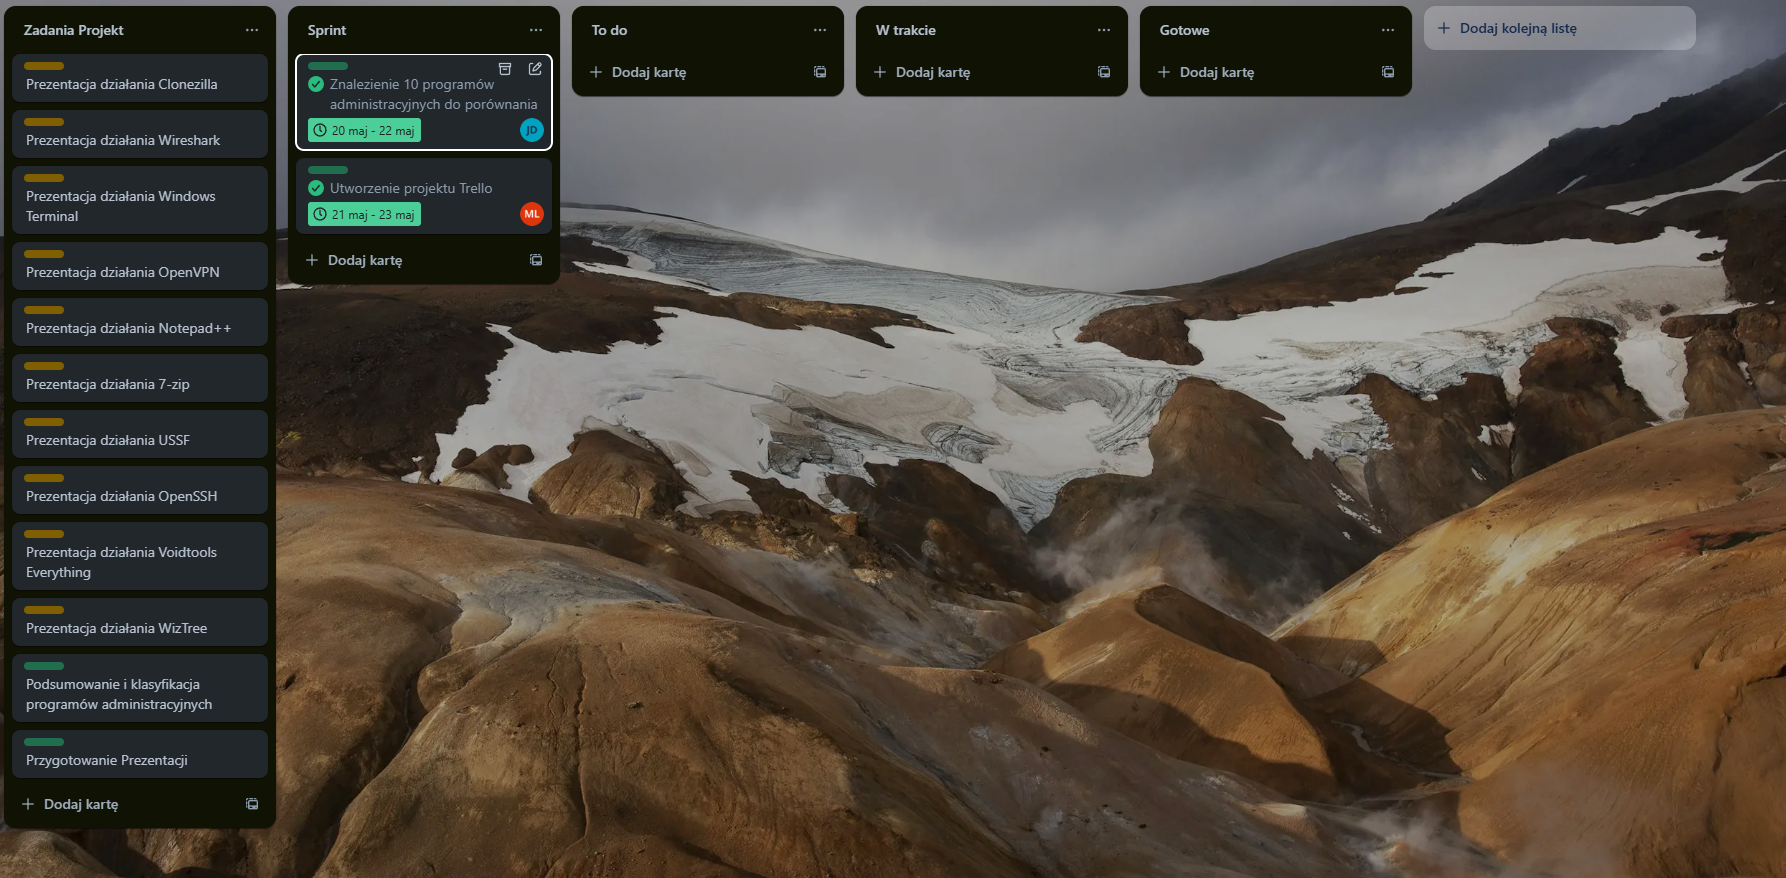
\includegraphics[width=0.8\linewidth]{media/Trello_screeny/Sprint1.PNG}
        \caption[sprint1]{Sprint 1 - Wybranie programów i stworzenie projektu Trello}
        \label{fig:sprint1}
    \end{figure}
    
\subsubsection{Sprint 2}

    \begin{figure}[H]
        \centering
        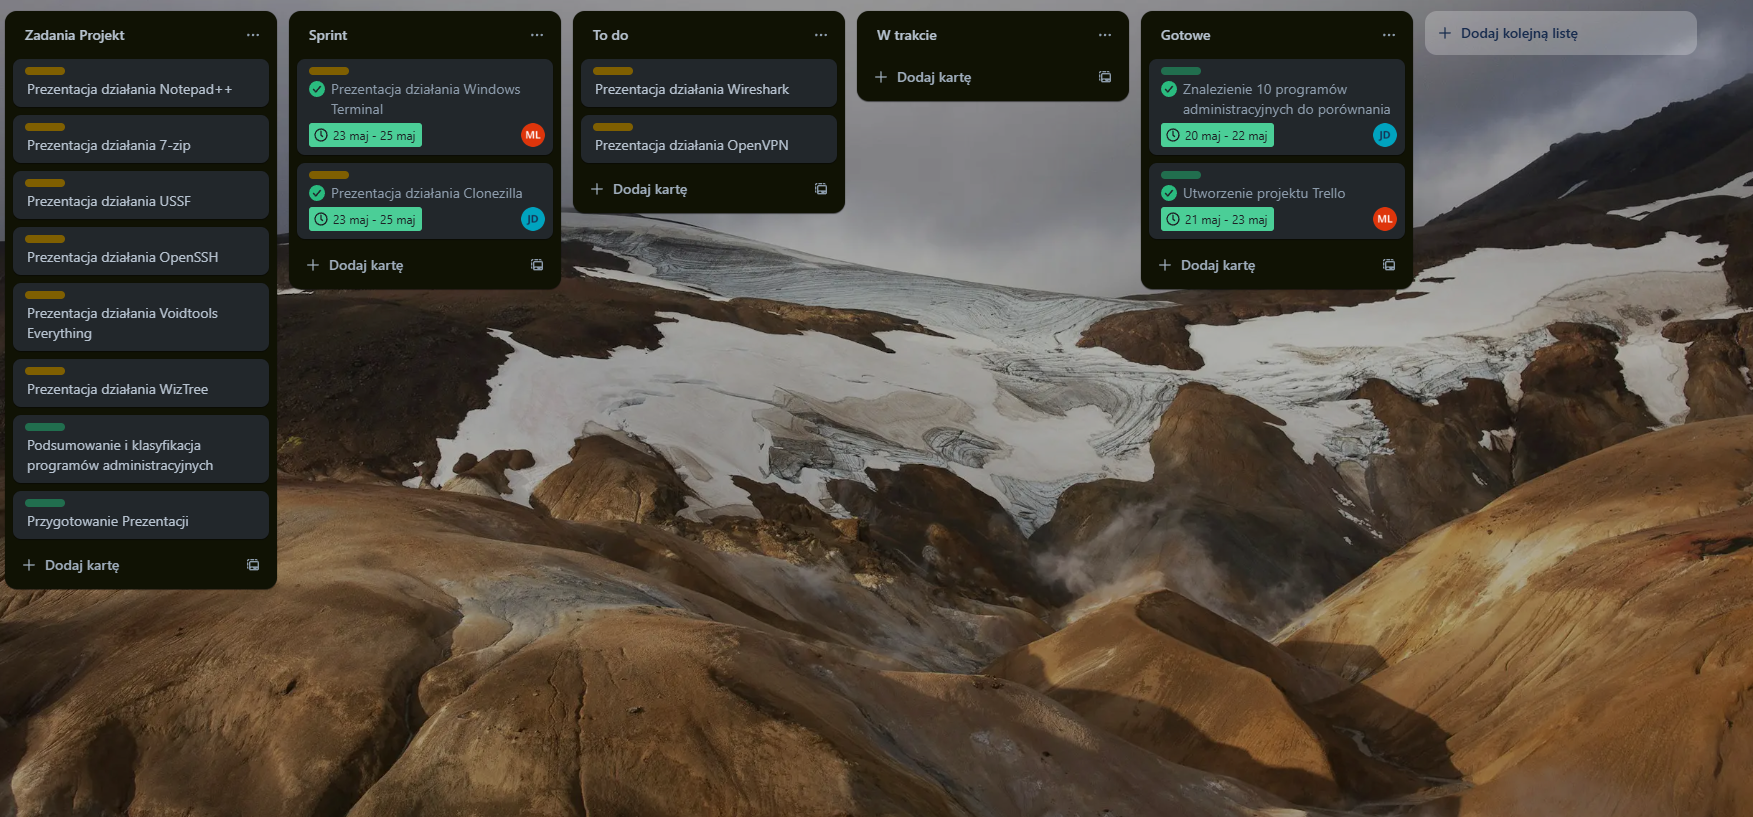
\includegraphics[width=0.8\linewidth]{media/Trello_screeny/Sprint2_1.PNG}
        \caption[Sprint2.1]{Sprint 2.1 - Windows Terminal, Clonezilla}
        \label{fig:sprint2_1}
    \end{figure}

    \begin{figure}[H]
        \centering
        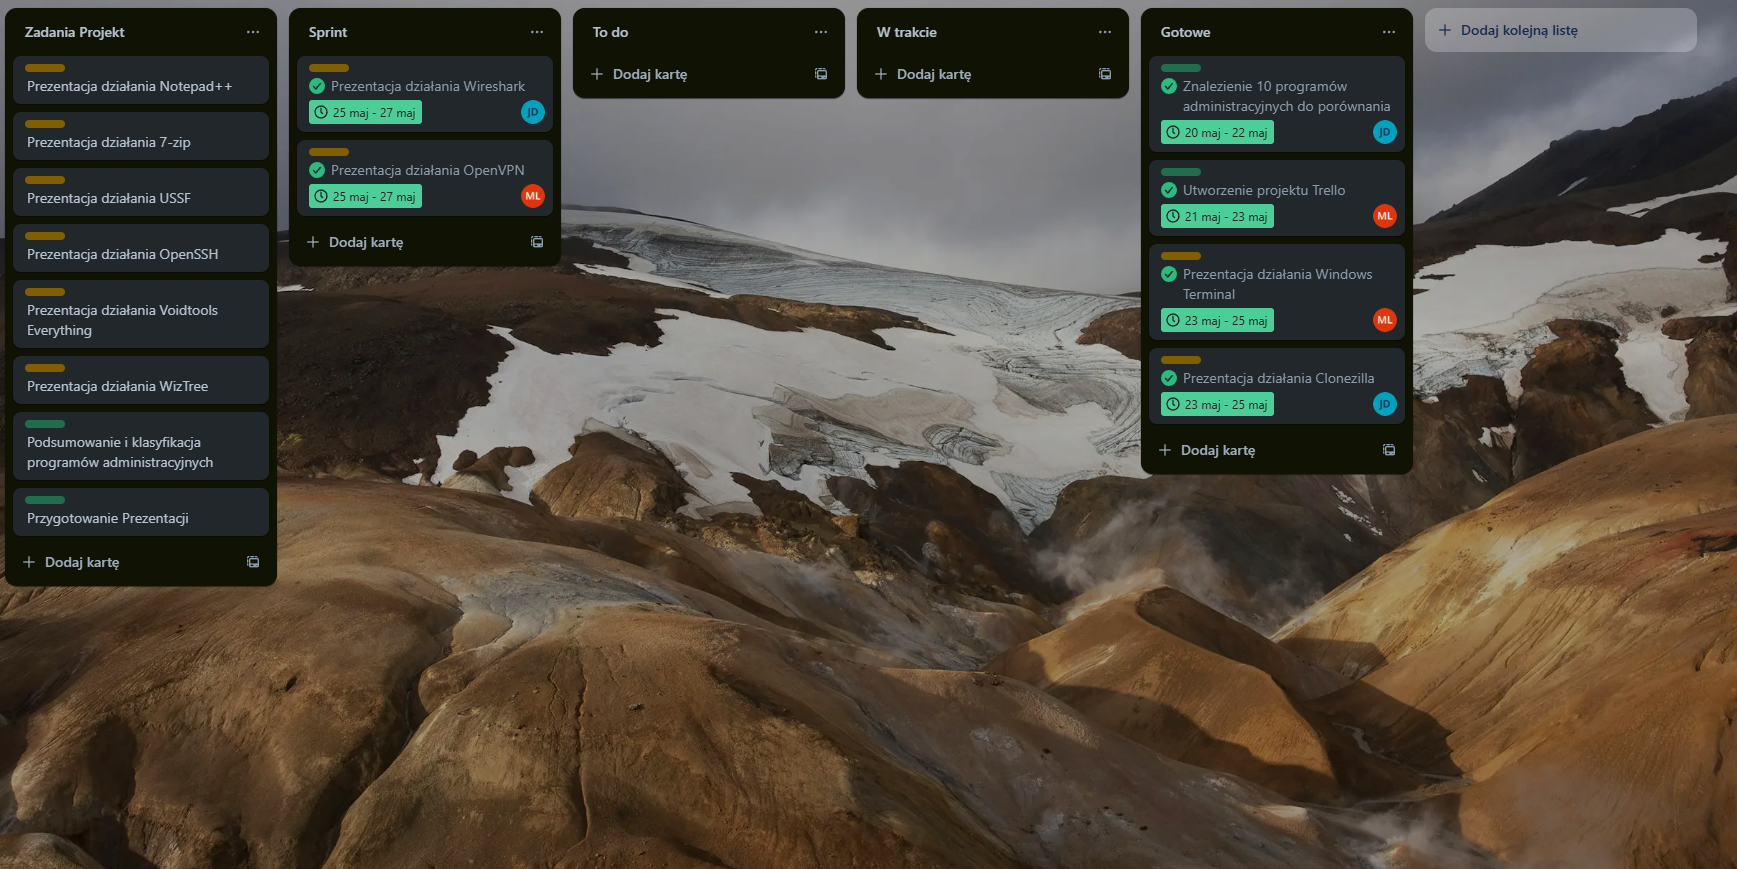
\includegraphics[width=0.8\linewidth]{media/Trello_screeny/Sprint2_2.PNG}
        \caption[Sprint2.2]{Sprint 2.2 - Wireshark, OpenVPN}
        \label{fig:sprint2_2}
    \end{figure}
    
\subsubsection{Sprint 3}

    \begin{figure}[H]
        \centering
        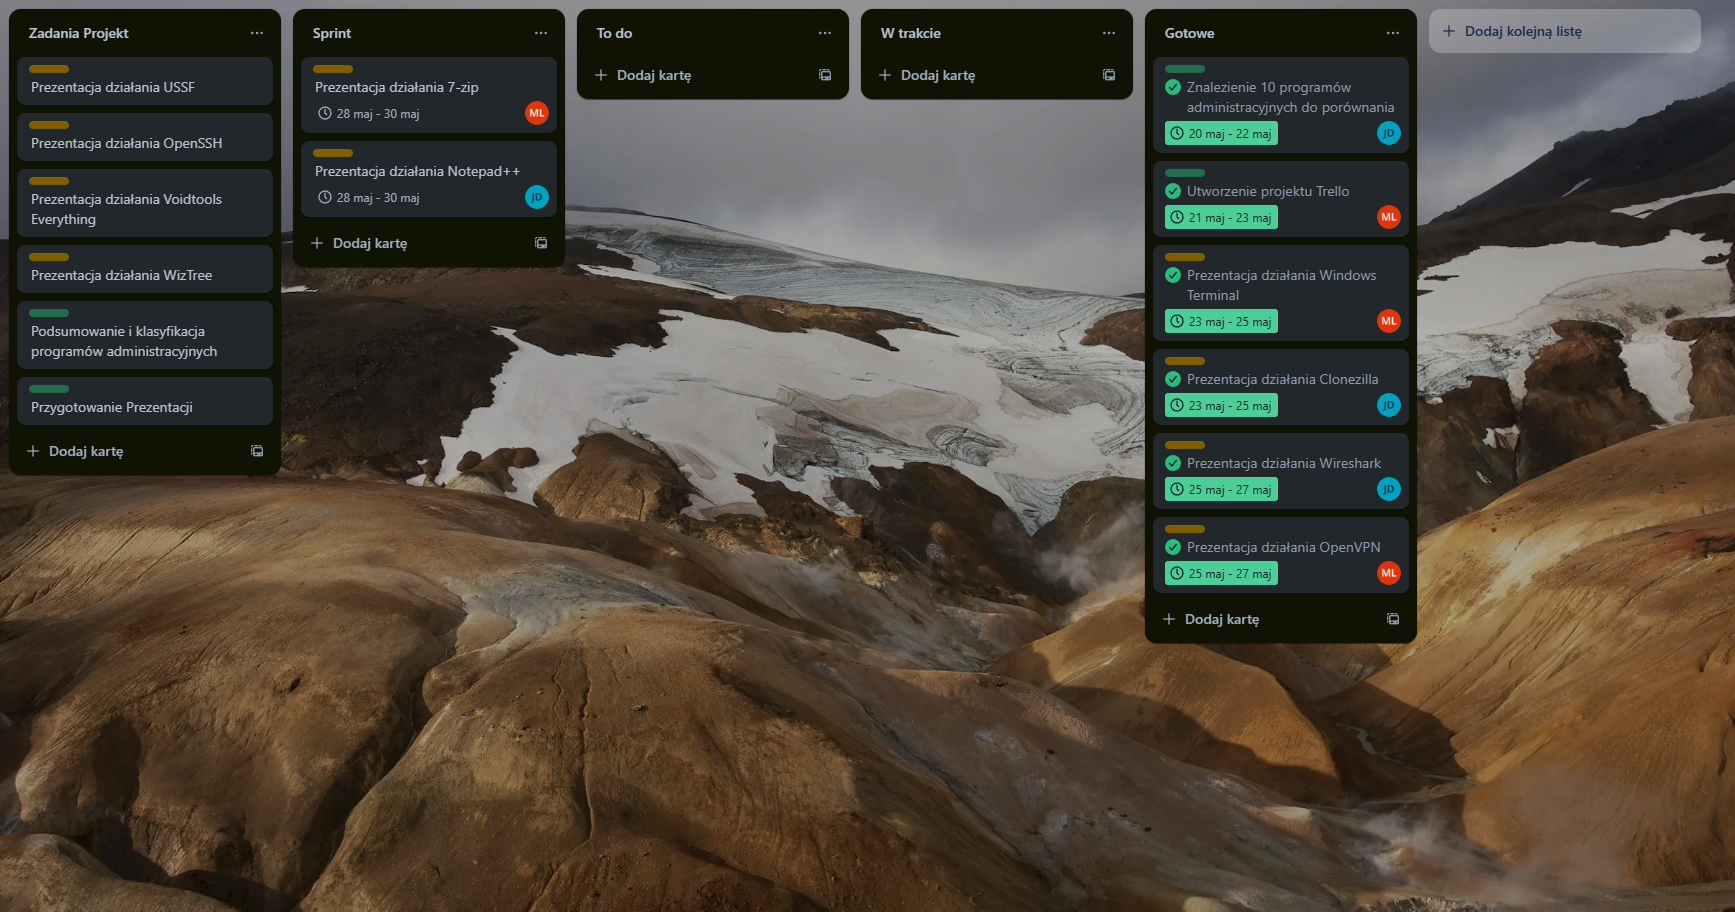
\includegraphics[width=0.8\linewidth]{media/Trello_screeny/Sprint3.PNG}
        \caption[Sprint3]{Sprint 3 - 7-Zip, Notepad++}
        \label{fig:sprint3}
    \end{figure}
    
\subsubsection{Sprint 4}

    \begin{figure}[H]
        \centering
        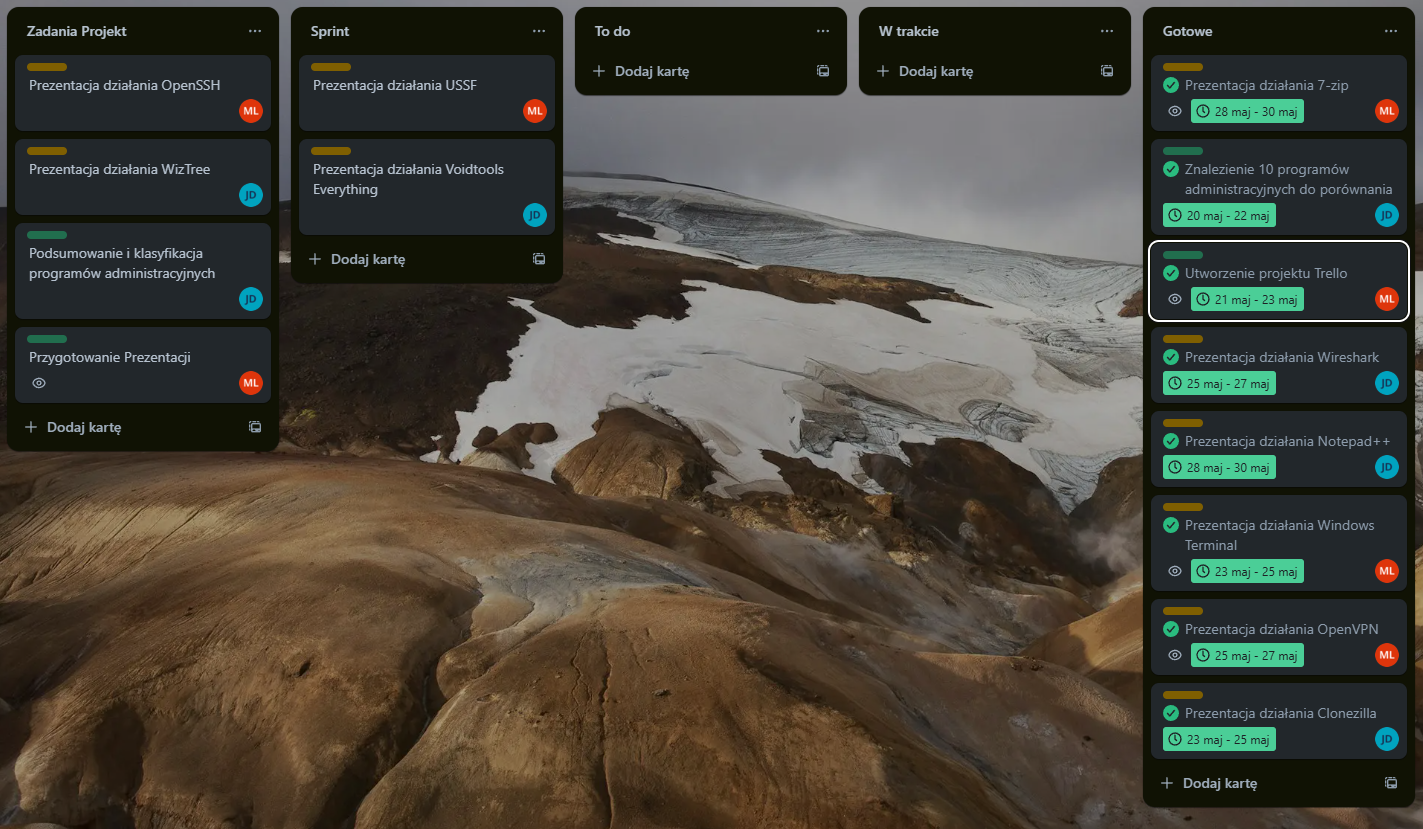
\includegraphics[width=0.8\linewidth]{media/Trello_screeny/Sprint5.PNG}
        \caption[Sprint4]{Sprint 4 - USSF, Voidtools Everything}
        \label{fig:sprint4}
    \end{figure}
    
\subsubsection{Sprint 5}

    \begin{figure}[H]
        \centering
        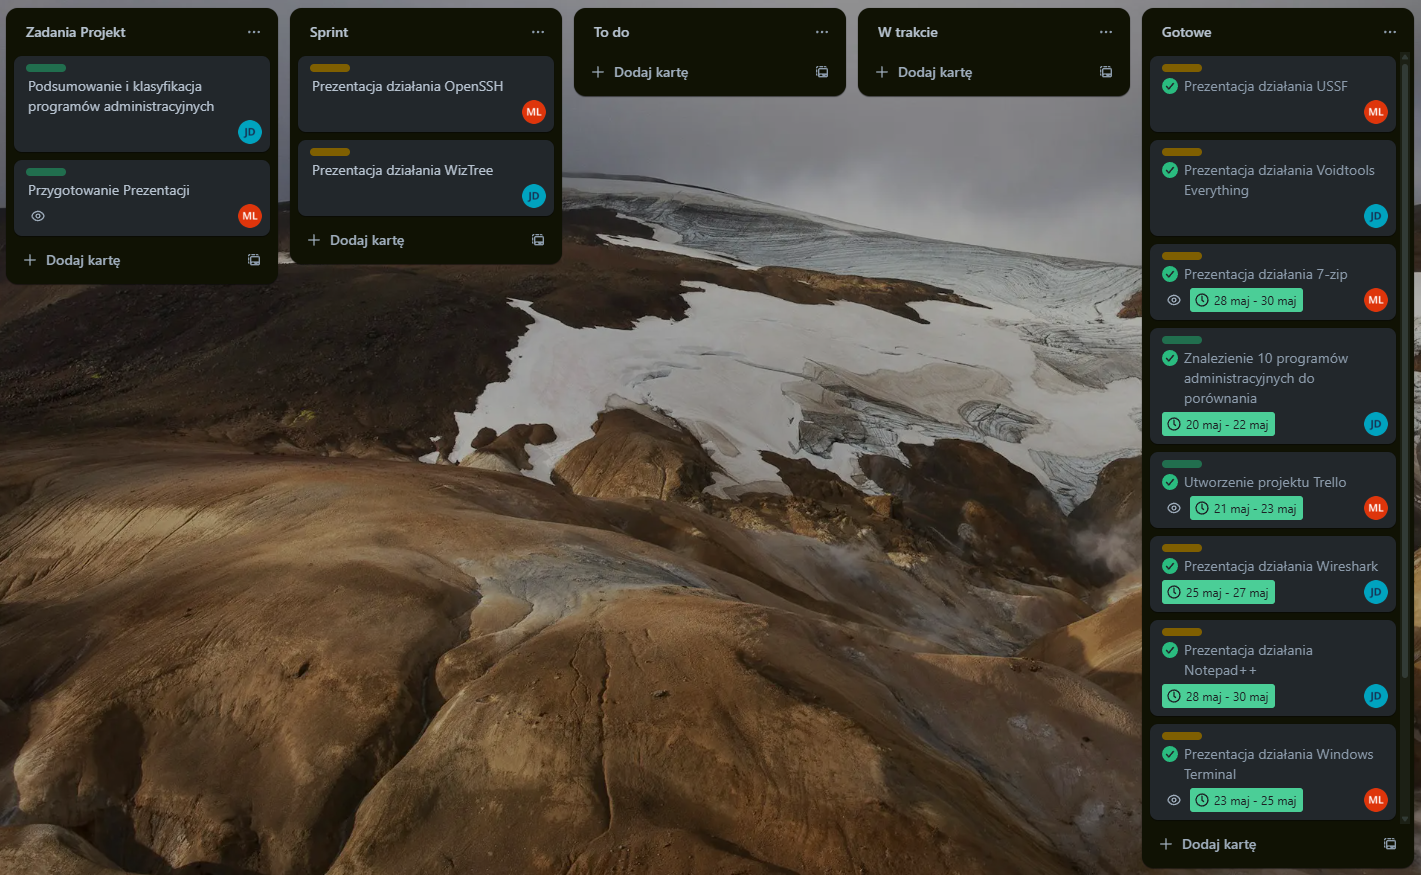
\includegraphics[width=0.8\linewidth]{media/Trello_screeny/Sprint6.png}
        \caption[Sprint5]{Sprint 5 - OpenSSH, WizTree}
        \label{fig:sprint5}
    \end{figure}
    
\subsubsection{Sprint 6}

    \begin{figure}[H]
        \centering
        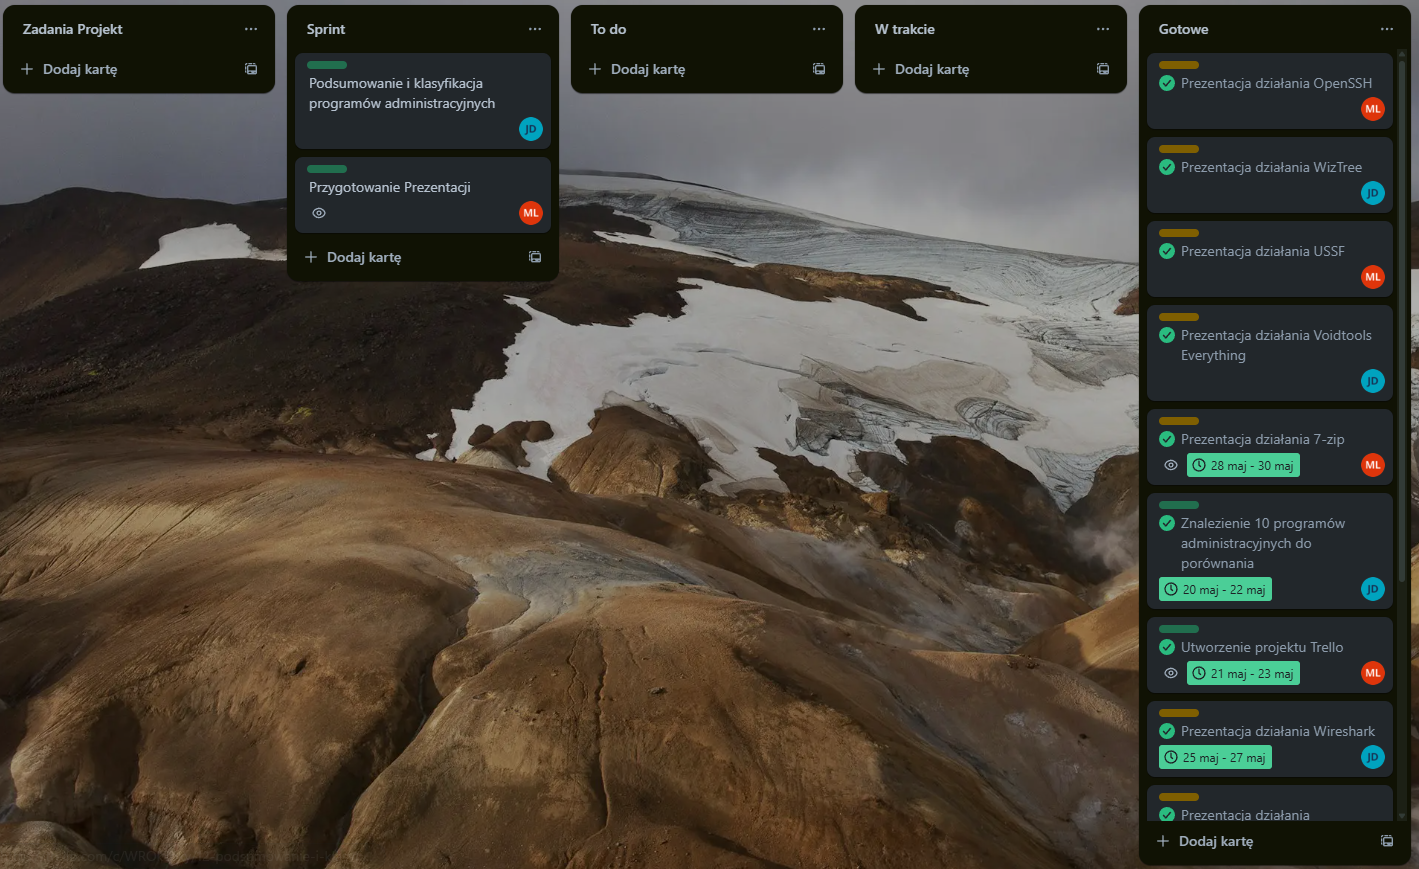
\includegraphics[width=0.8\linewidth]{media/Trello_screeny/Sprint7.PNG}
        \caption[Sprint6]{Sprint 6 - Klasyfikacja programów, przygotowanie dokumentacji oraz prezentacji}
        \label{fig:sprint6}
    \end{figure}

\newpage
\subsection{Opis narzędzi}

\subsubsection{OpenSSH}
    Niezawodne narzędzie do zdalnego zarządzania systemami poprzez protokół SSH. Umożliwia bezpieczne logowanie i przesyłanie plików.
    \\
    Aby SSH poprawnie działało należy upewnić się czy w systemie operacyjnym zainstalowana jest usługa SSH Server oraz Client.
    \begin{figure}[H]
        \centering
        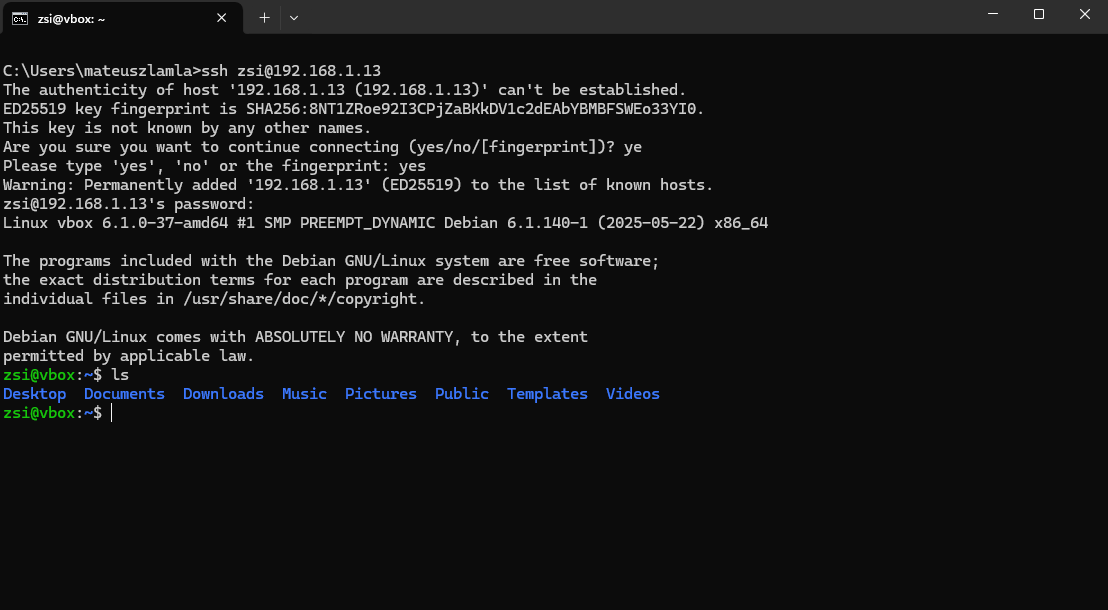
\includegraphics[width=0.8\linewidth]{media/OpenSSH/1_poloczenie.png}
        \caption[polaczenie ssh]{Połączenie dwóch systemów przez SSH}
        \label{fig:ssh_polaczenie}
    \end{figure}

    \begin{figure}[H]
        \centering
        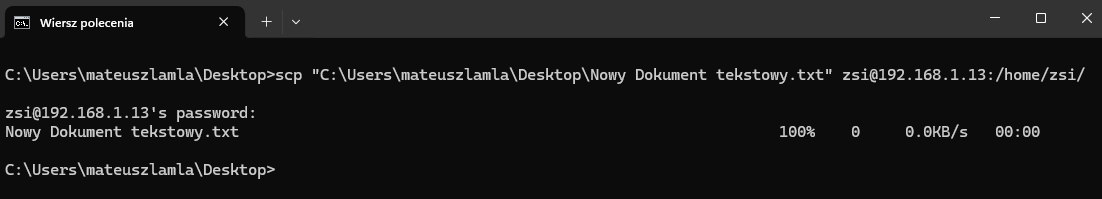
\includegraphics[width=0.8\linewidth]{media/OpenSSH/2_kopiowanie_plikow.png}
        \caption[kopiowanie ssh]{Przez protokół SSH możemy kopiować pliki pomiędzy dwoma systemami}
        \label{fig:ssh_kopiowanie}
    \end{figure}

    \begin{figure}[H]
        \centering
        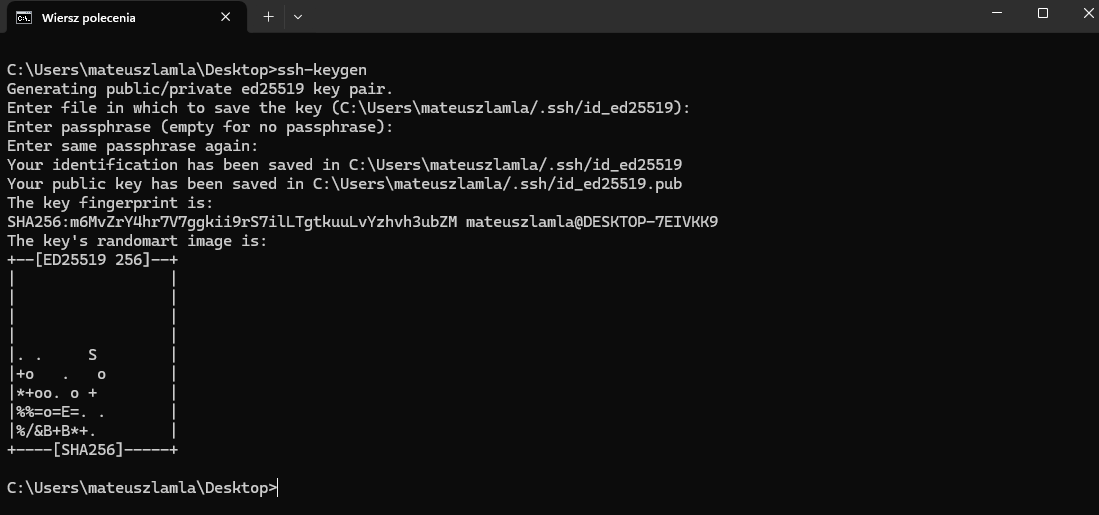
\includegraphics[width=0.8\linewidth]{media/OpenSSH/3_tworzenie_klucza.png}
        \caption[klucz ssh]{Wygenerowanie klucza do logowania}
        \label{fig:ssh_klucz}
    \end{figure}

    \begin{figure}[H]
        \centering
        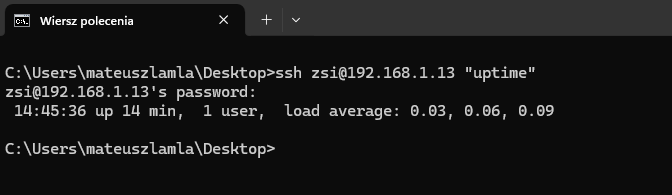
\includegraphics[width=0.8\linewidth]{media/OpenSSH/4_zdalne wykonywanie_polecenia.png}
        \caption[zdalne polecenie ssh]{OpenSSH oferuje również opcję zdalengo wykonania polecenia}
        \label{fig:ssh_polecenie_zdalne}
    \end{figure}

    \begin{figure}[H]
        \centering
        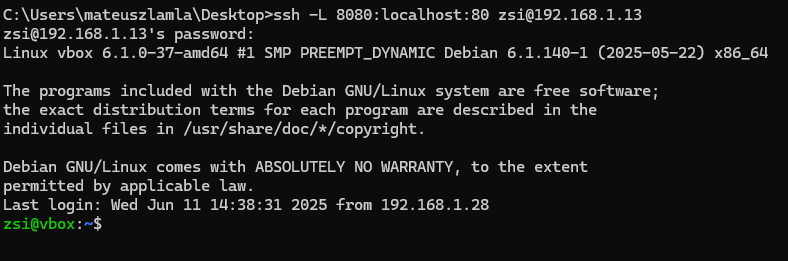
\includegraphics[width=0.8\linewidth]{media/OpenSSH/5_tunelowanie_portu.png}
        \caption[tunelowanie portu ssh]{Mamy również opcję tunelowania portu w celu przekierowania ruchu sieciowego przez bezpieczne, szyfrowane połączenie SSH}
        \label{fig:ssh_tunelowanie_portu}
    \end{figure}

    \begin{figure}[H]
        \centering
        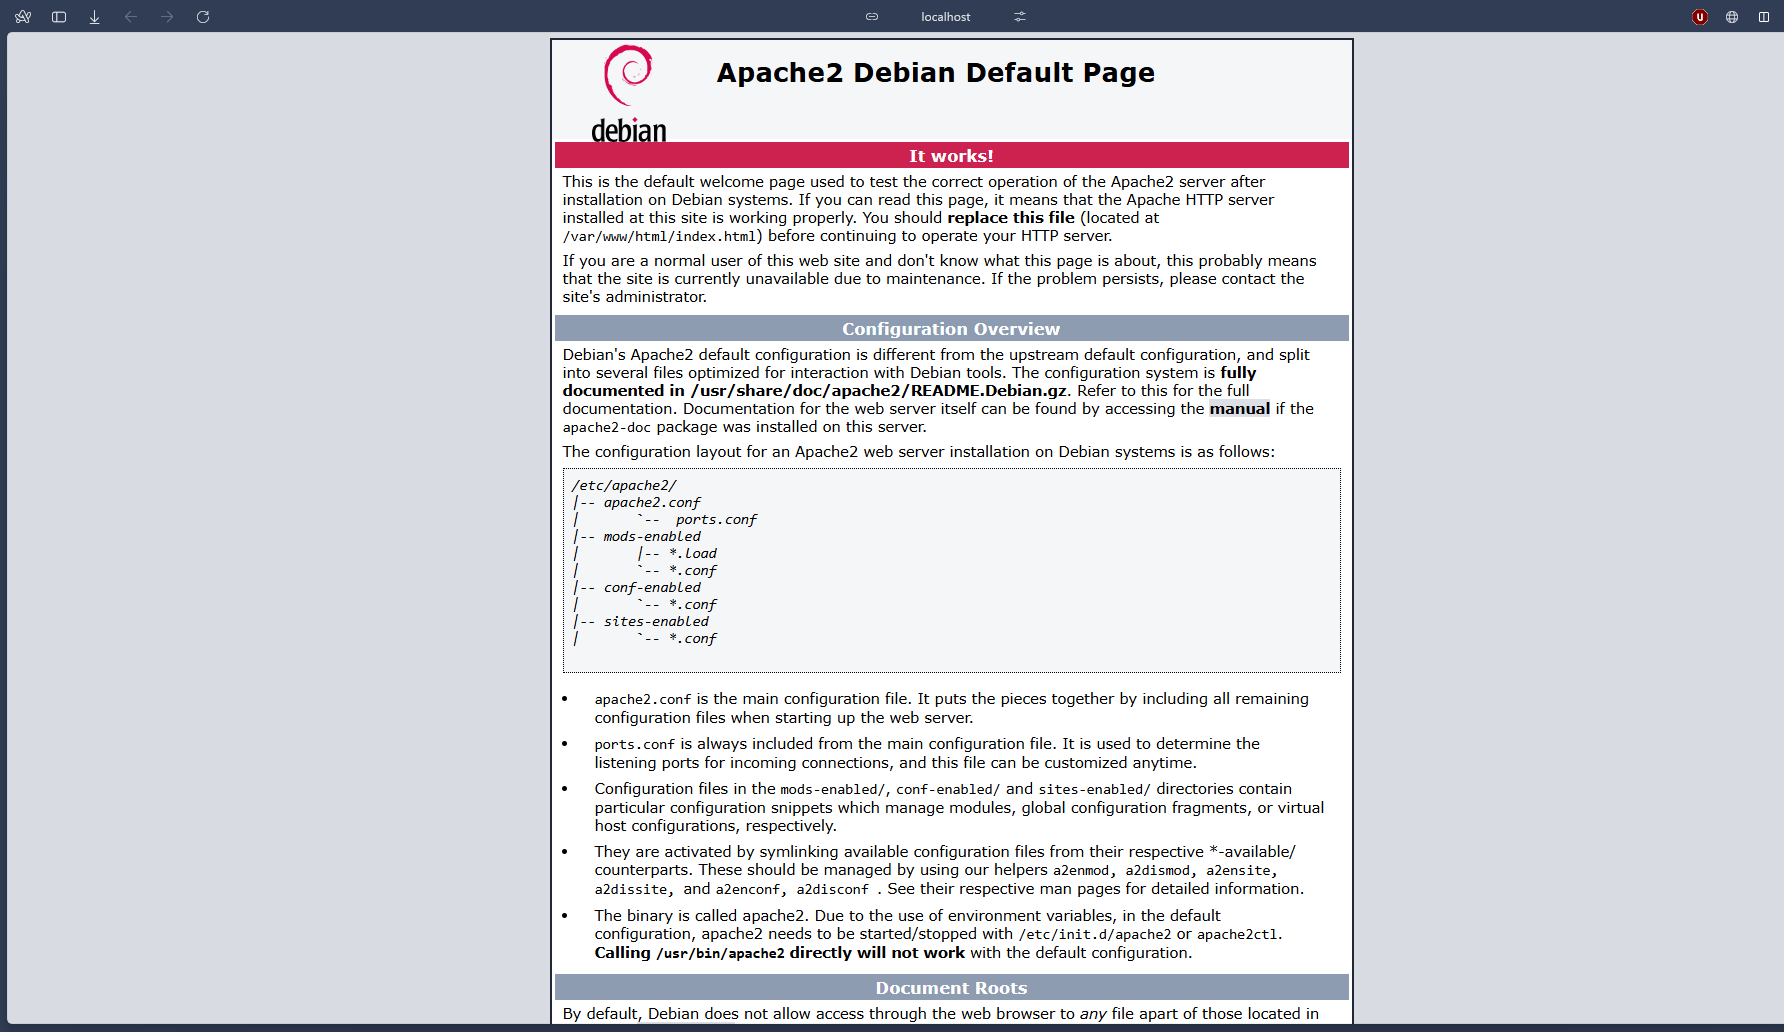
\includegraphics[width=0.8\linewidth]{media/OpenSSH/5_1_localhost_z_debiana_na_windowsie.png}
        \caption[pokazanie localhost ssh]{Wyświetlenie localhosta przez SSH z drugiego systemu}
        \label{fig:ssh_localhost}
    \end{figure}

    \begin{figure}[H]
        \centering
        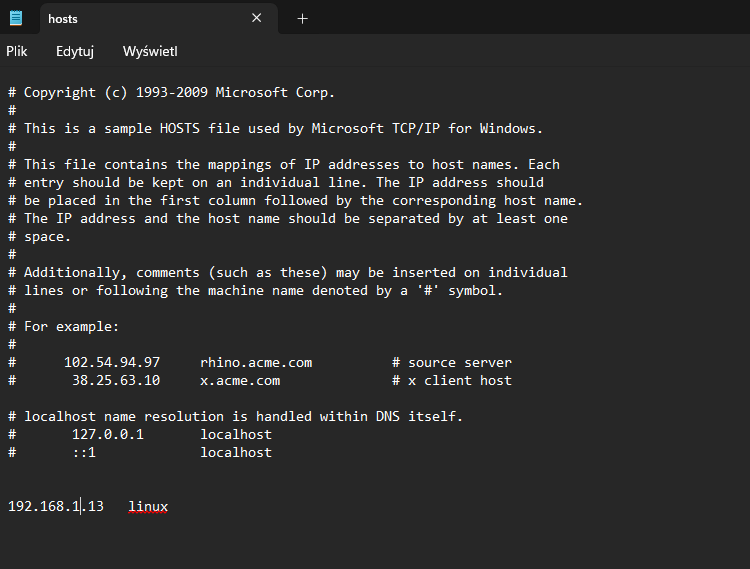
\includegraphics[width=0.8\linewidth]{media/OpenSSH/6_edycja_hosts.png}
        \caption[edycja hosts ssh]{Aby ułatwić łączenie się możemy wyedytować plik hosts aby zamiast IP używać nazw urządzeń}
        \label{fig:ssh_edycja_hosts}
    \end{figure}

    \begin{figure}[H]
        \centering
        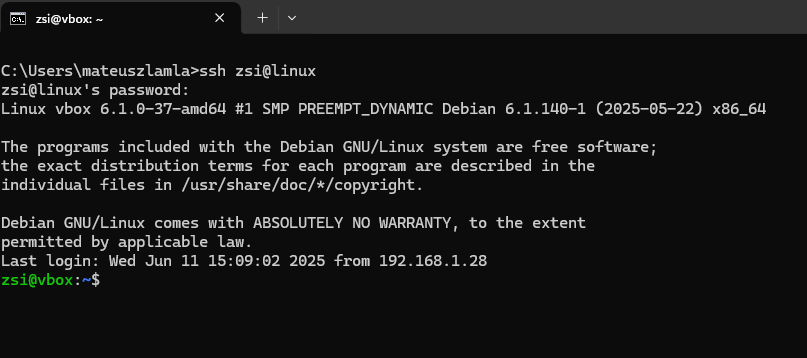
\includegraphics[width=0.8\linewidth]{media/OpenSSH/7_logowanie_po_nazwie_a_nie_po_ip.png}
        \caption[Logowanie po nazwie ssh]{Logowanie do drugiego systemu za pomocą nazwy, a nie IP}
        \label{fig:logowanie_nazwa}
    \end{figure}
    
    Alternatywą dla OpenSSH może być program \textbf{PuTTY}. OpenSSH jest lepsze do pracy na serwerach, natomiast PuTTY sprawdzi się lepiej dla użytkowników preferujących GUI.
\newpage
\subsubsection{Everything (Voidtools)}
    Błyskawiczna wyszukiwarka plików w systemie Windows. Niezastąpiona w sytuacjach, gdy administrator musi szybko zlokalizować określone dane.
    
    \begin{figure}[H]
        \centering
        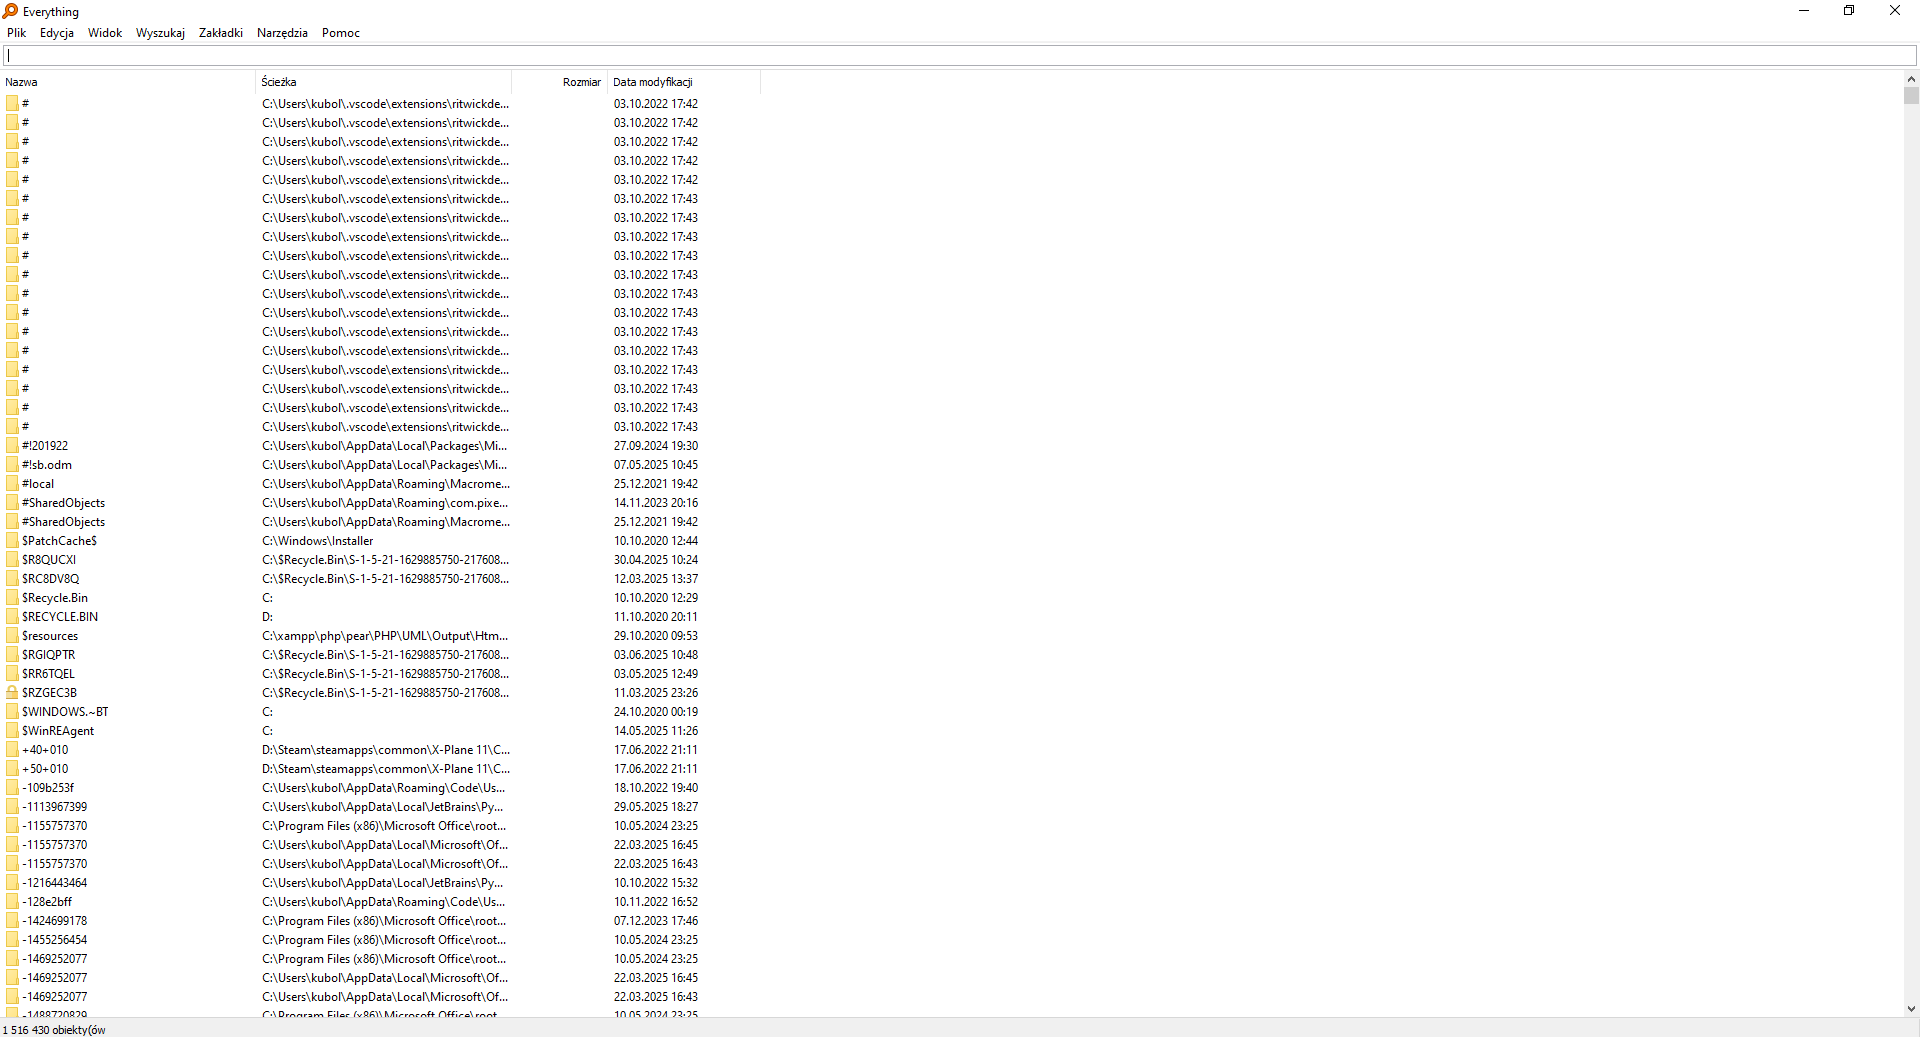
\includegraphics[width=0.8\linewidth]{media/EverythingTool/ev1.PNG}
        \caption[Everything glowne]{Strona początkowa programu po wczytaniu danych z dysku}
        \label{fig:ev_glowna}
    \end{figure}
    
    \begin{figure}[H]
        \centering
        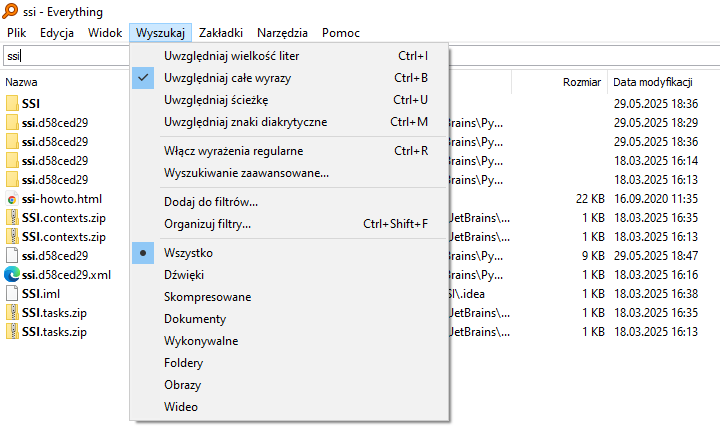
\includegraphics[width=0.8\linewidth]{media/EverythingTool/ev2.png}
        \caption[everything filtr slowa]{Wyszukiwanie plików zawierających całe wpisane słowo}
        \label{fig:ev_slowo}
    \end{figure}

    \begin{figure}[H]
        \centering
        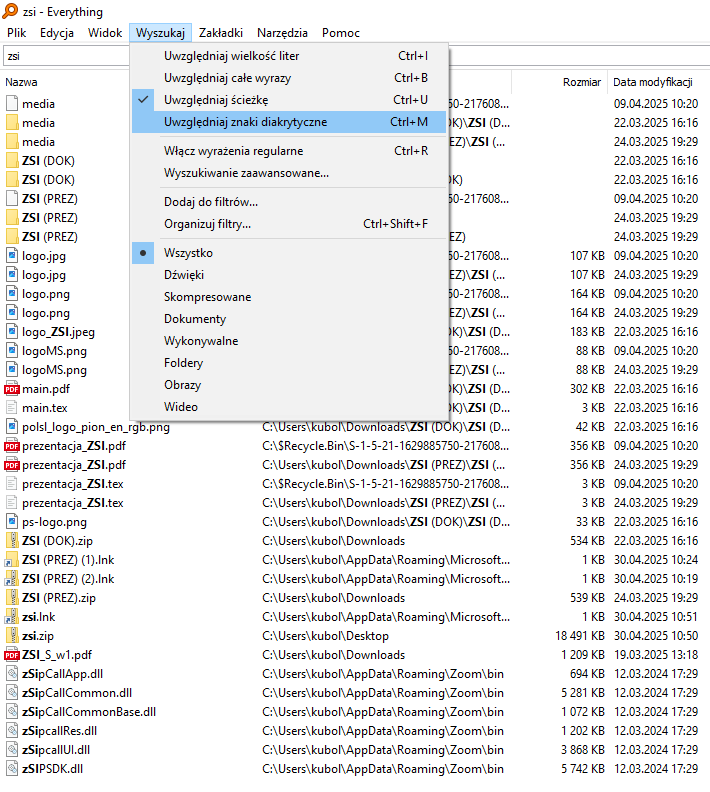
\includegraphics[width=0.8\linewidth]{media/EverythingTool/ev3.png}
        \caption[everything filtr sciezka]{Wyszukiwanie plików po zarówno nazwie jak i ścieżce}
        \label{fig:ev_sciezka}
    \end{figure}

    \begin{figure}[H]
        \centering
        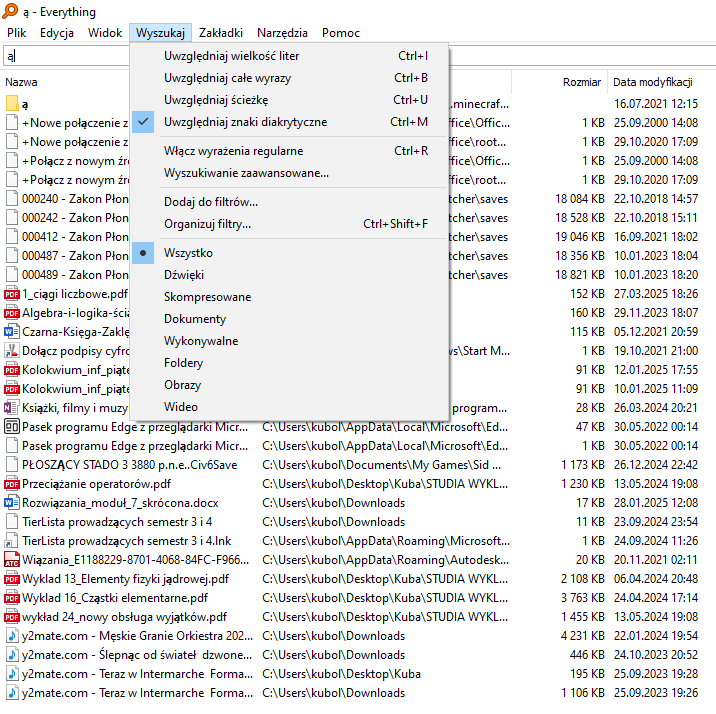
\includegraphics[width=0.8\linewidth]{media/EverythingTool/ev4.png}
        \caption[everything znaki diakrytyczne]{Wyszukiwanie z uwzględnieniem znaków diakrytycznych}
        \label{fig:ev_diakr}
    \end{figure}

    \begin{figure}[H]
        \centering
        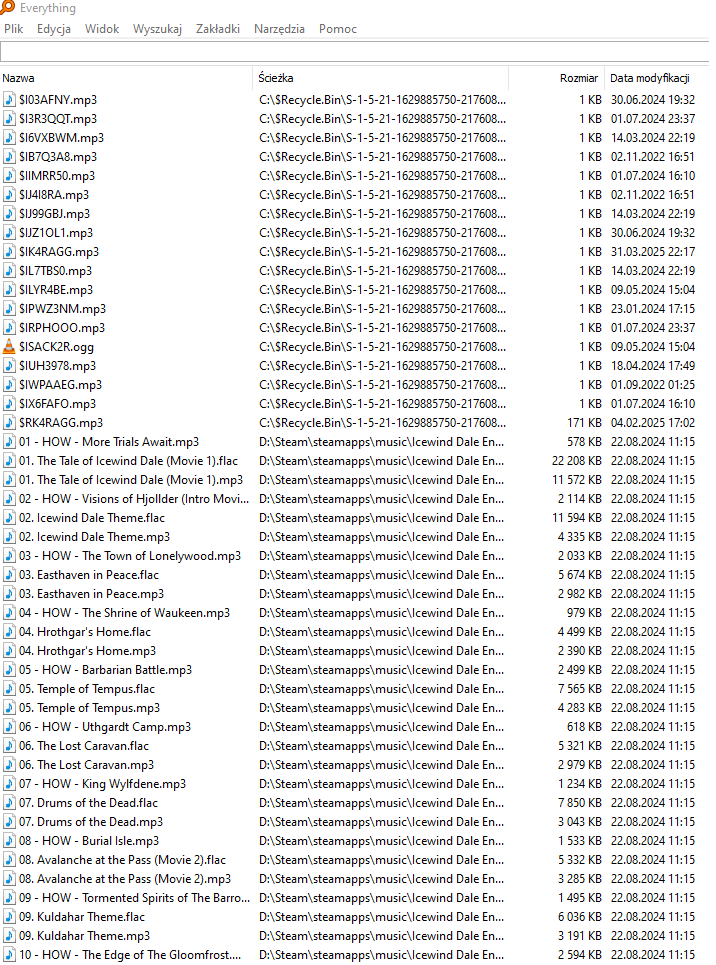
\includegraphics[width=0.8\linewidth]{media/EverythingTool/ev5.png}
        \caption[everything typ]{Wyszukiwanie jedynie plików z określonym rozszerzeniem}
        \label{fig:ev_rozszerz}
    \end{figure}

    \begin{figure}[H]
        \centering
        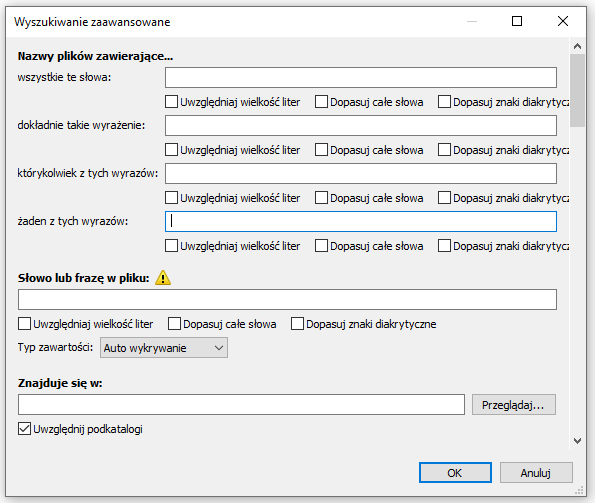
\includegraphics[width=0.8\linewidth]{media/EverythingTool/ev6.PNG}
        \caption[everything filtrowanie dokladne]{Możliwość wyszukiwania plików za pomocą wielu parametrów np. paru słów lub w określonym miejscu na dysku}
        \label{fig:ev_param}
    \end{figure}

    \begin{figure}[H]
        \centering
        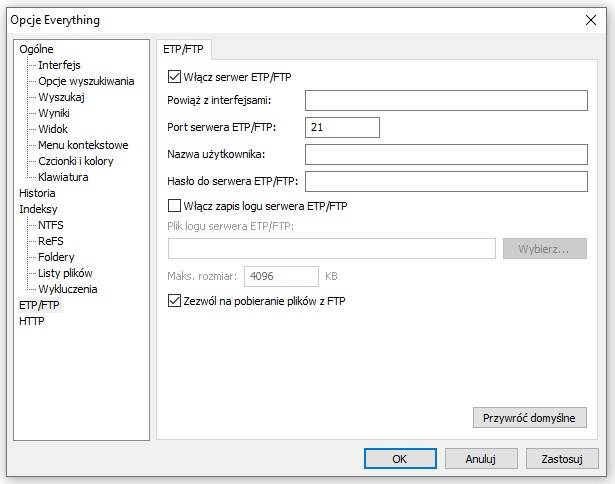
\includegraphics[width=0.8\linewidth]{media/EverythingTool/ev7.PNG}
        \caption[everything ftp]{Możliwość połączenia się do dysku innego hosta za pomocą FTP lub utworzenia serwera na swoim komputerze, aby można było łączyć się do nas}
        \label{fig:ev_ftp}
    \end{figure}
    Podobnym programem do Everything (Void Tools) jest \textbf{UltraSearch}, który pomimo posiadania paru bardziej zaawansowanych opcji jest znacząco wolniejszy od wybranego przez nas programu. Prędkość działania w przypadku oprogramowania tego typu jest kluczową cechą, jako że chcemy znajdować pliki najszybciej i najskuteczniej jak tylko się da. Wybrany przez nas program jest niezastąpionym narzędziem do codziennego użytku dzięki swojej prostocie.
    
\subsubsection{WizTree}
    Wizualizuje strukturę zajętości dysku, ułatwiając zarządzanie przestrzenią dyskową.
    \begin{figure}[H]
        \centering
        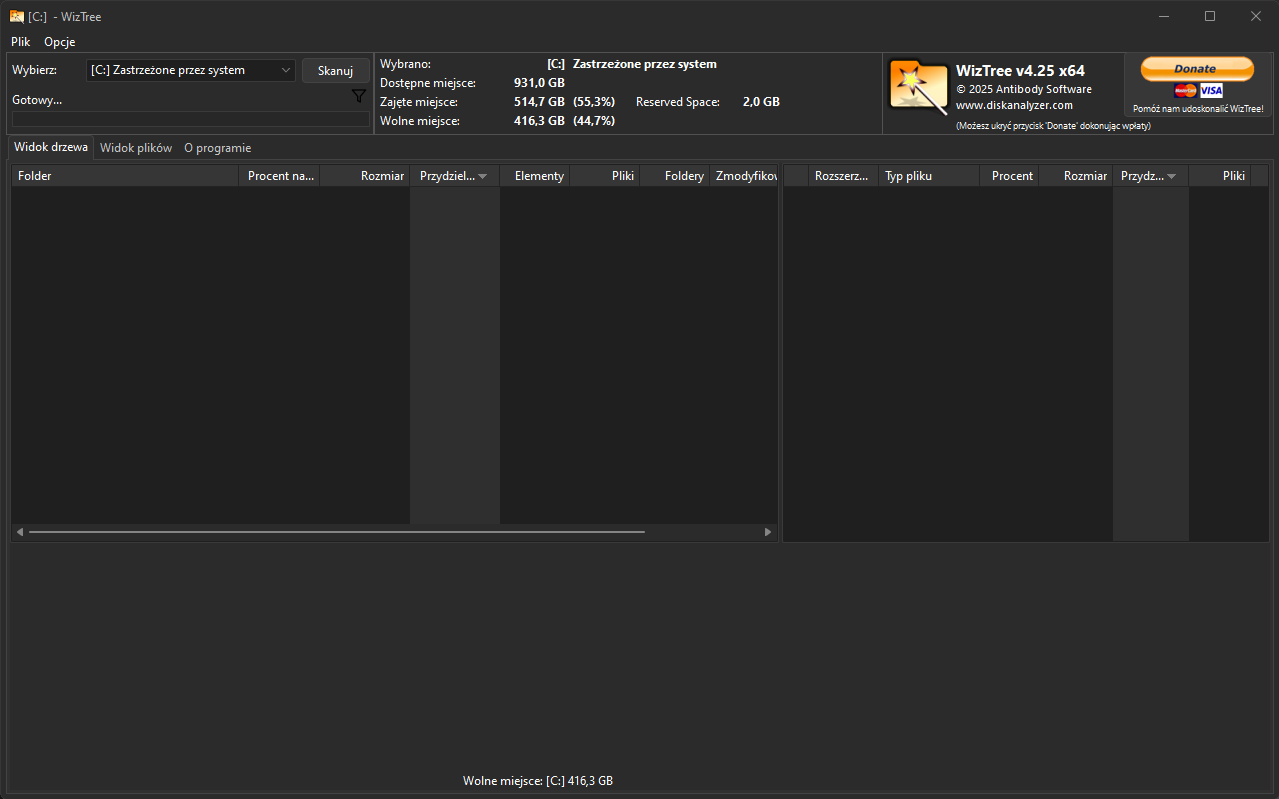
\includegraphics[width=0.8\linewidth]{media/WizTree/wiz1.PNG}
        \caption[wiz glowne]{Strona początkowa programu pokazująca podstawowe informacje o przestrzeni dyskowej na wybranym nośniku}
        \label{fig:wiz_glowne}
    \end{figure}

    \begin{figure}[H]
        \centering
        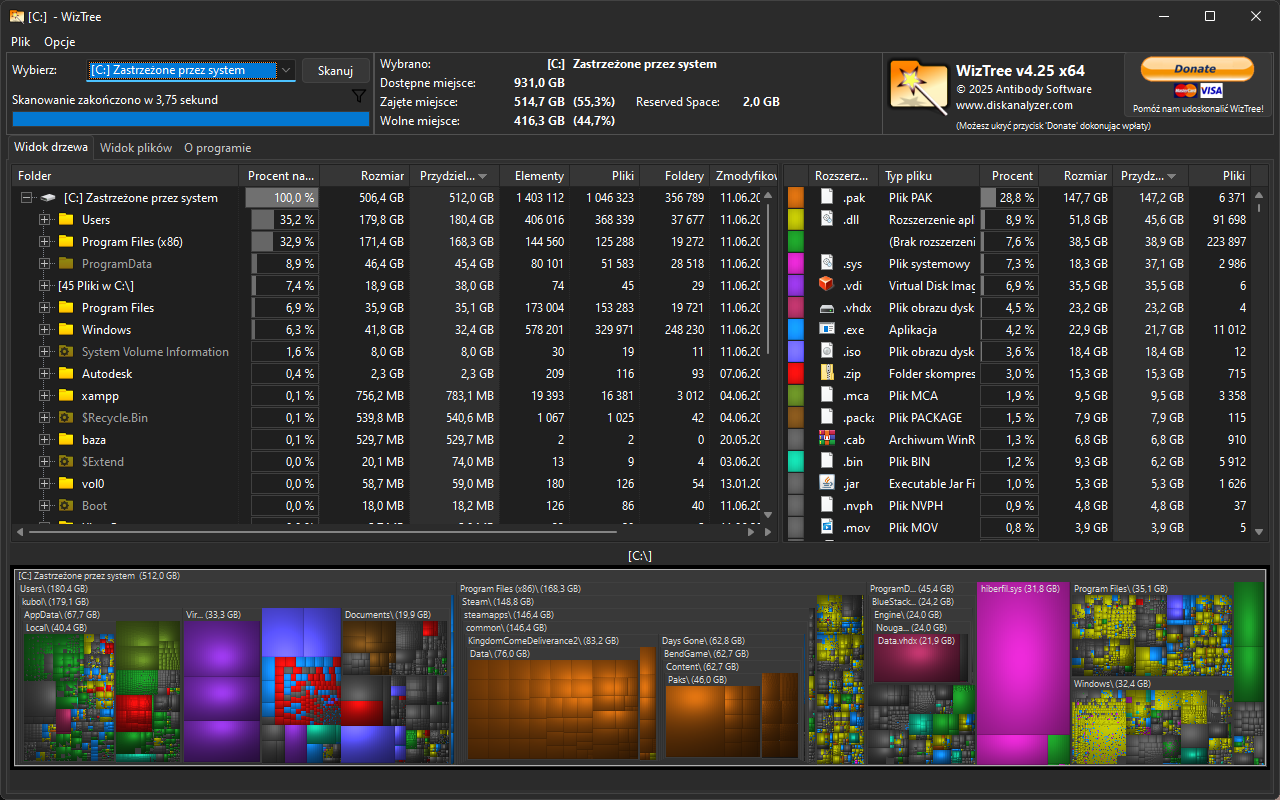
\includegraphics[width=0.8\linewidth]{media/WizTree/wiz2.PNG}
        \caption[wiz przeskanowane]{Statystyki, wizualizacje oraz rozbudowany eksplorator plików po przeskanowaniu dysku programem}
        \label{fig:wiz_skan}
    \end{figure}

    \begin{figure}[H]
        \centering
        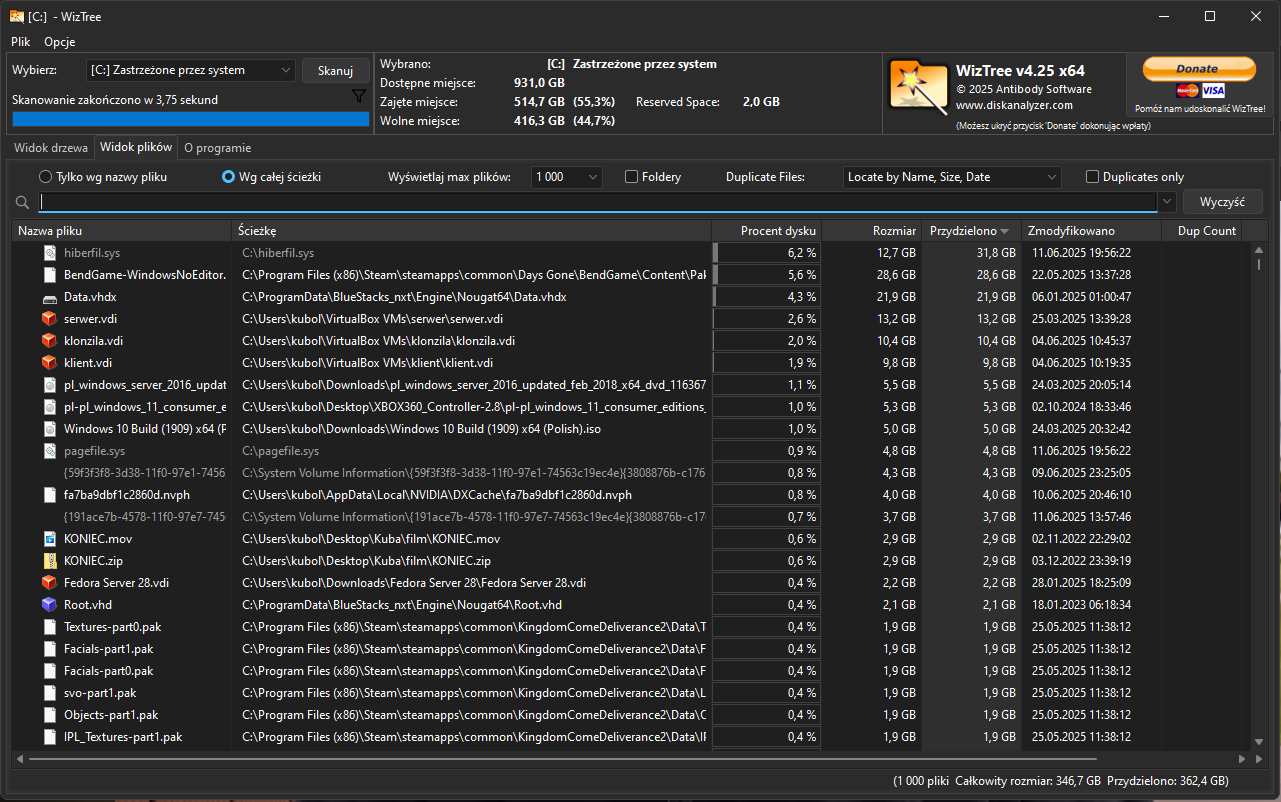
\includegraphics[width=0.8\linewidth]{media/WizTree/wiz3.PNG}
        \caption[wiz sciezki]{Możliwość wyświetlenia plików na podstawie miejsca, które mają przydzielone na dysku, co ułatwia porządkowanie dysku z obszernych i niepotrzebnych plików}
        \label{fig:wiz_sciezki}
    \end{figure}
    
    \begin{figure}[H]
        \centering
        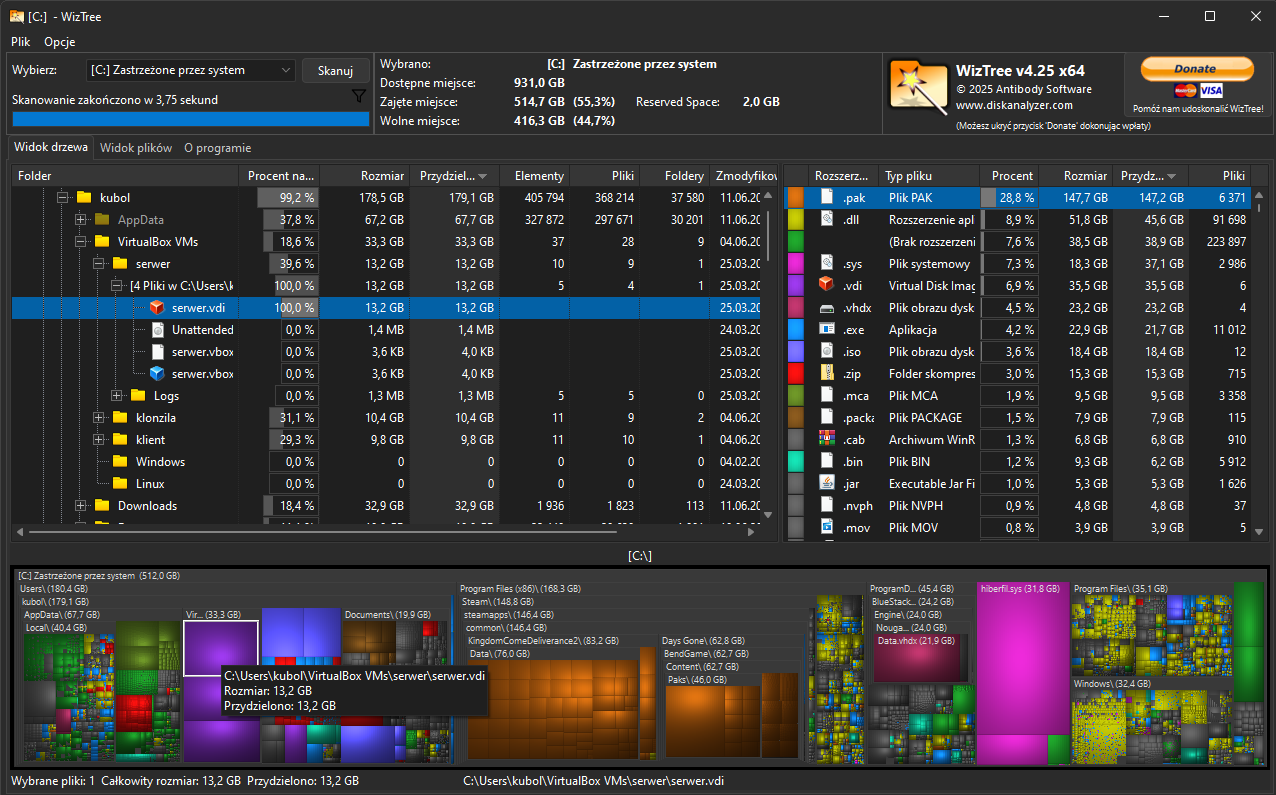
\includegraphics[width=0.8\linewidth]{media/WizTree/wiz4.png}
        \caption[wiz wyszukiwanie kliknieciem]{Możliwość "przeskoczenia" do widoku pliku za pomocą wizualizacji dysku na dole ekranu}
        \label{fig:wiz_klik}
    \end{figure}

    \begin{figure}[H]
        \centering
        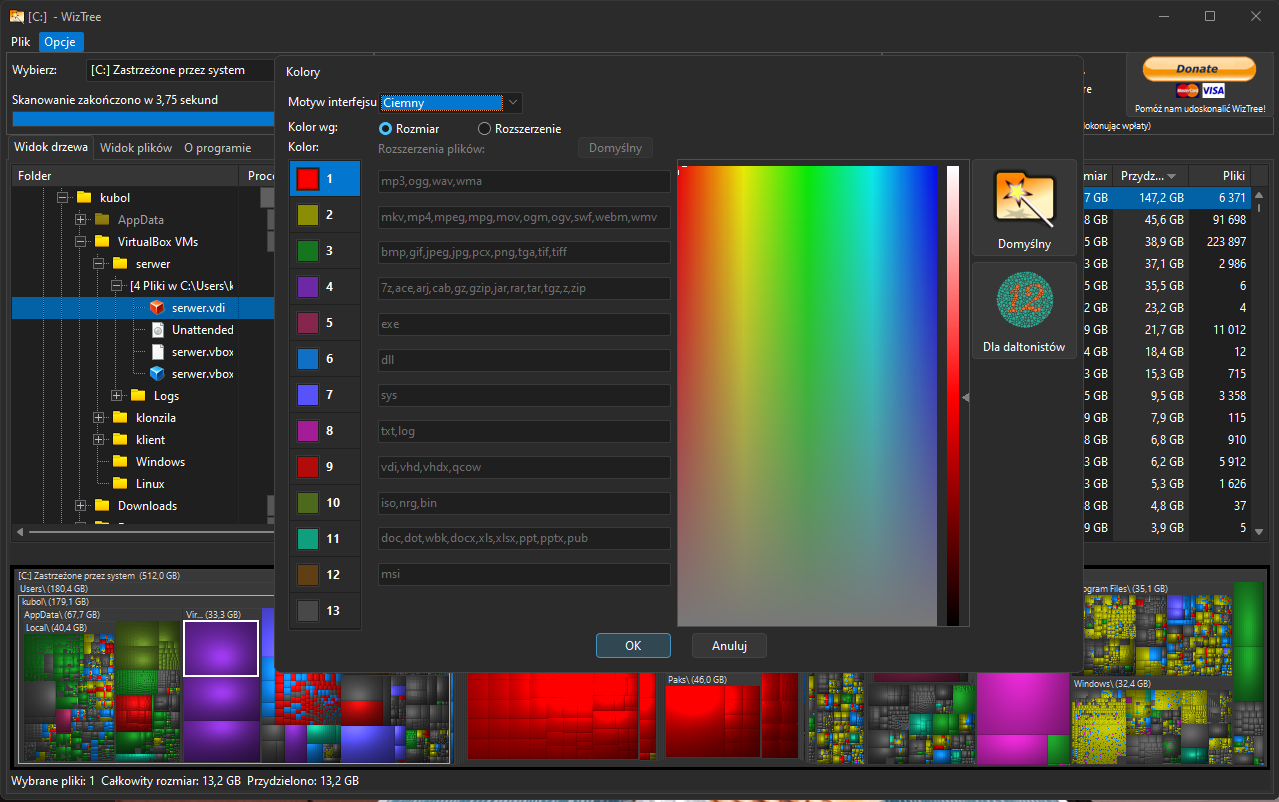
\includegraphics[width=0.8\linewidth]{media/WizTree/wiz5.PNG}
        \caption[wiz kolory]{Możliwość zmiany koloru dla danego rozszerzenia, w celu zwiększenia przejrzystości wizualizacji przestrzeni dyskowej dla użytkownika}
        \label{fig:wiz_kolory}
    \end{figure}

    \begin{figure}[H]
        \centering
        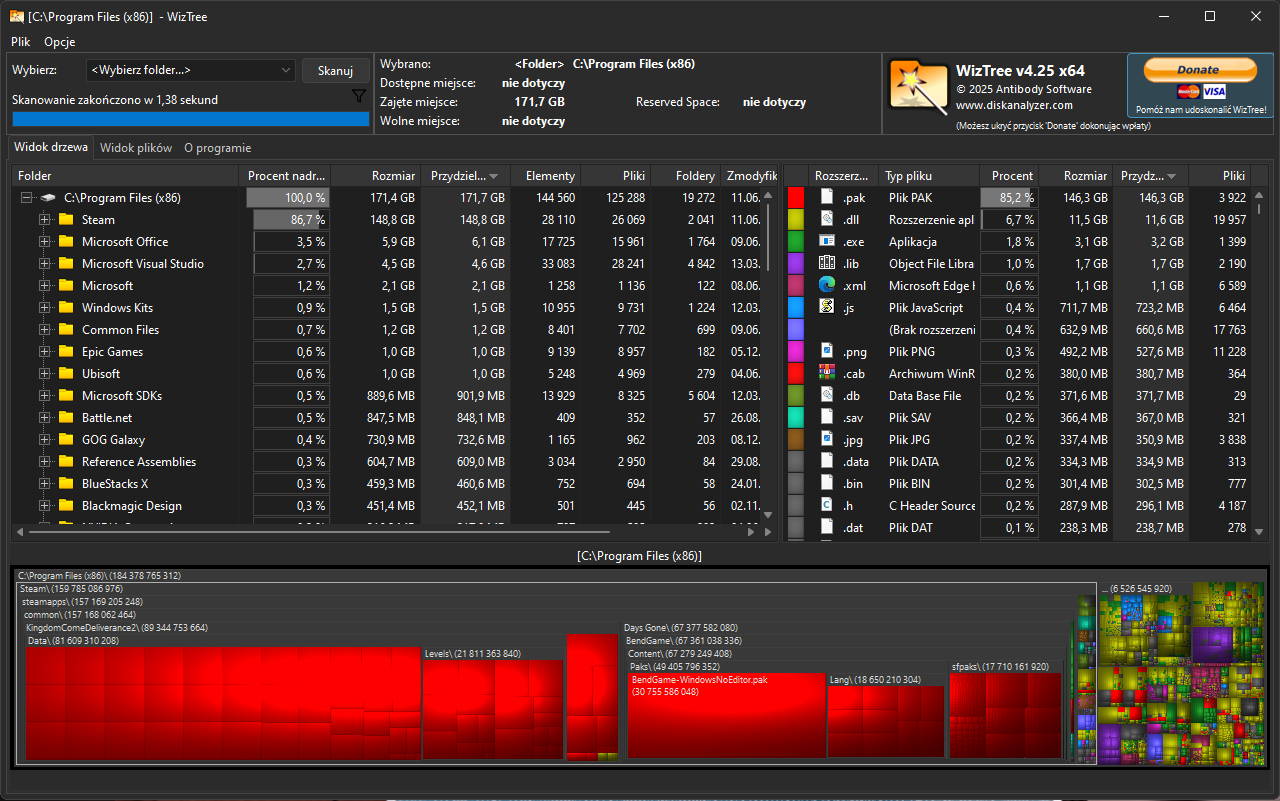
\includegraphics[width=0.8\linewidth]{media/WizTree/wiz6.PNG}
        \caption[wiz folder]{Możliwość przeskanowania jedynie wybranego folderu zamiast całości dysku}
        \label{fig:wiz_skan_folder}
    \end{figure}
    Alternatywą dla WizTree może być program \textbf{WinDirStat}, aczkolwiek WizTree działa zdecydowanie szybciej dzięki analizie MFT. WinDirStat skanuje pliki jeden po drugim, co znacząco spowalnia pracę.

\newpage
\subsubsection{USSF (Universal Silent Switch Finder)}
    Wykrywa przełączniki instalatorów w trybie cichym. Pomocne podczas automatyzowania instalacji oprogramowania.

    \begin{figure}[H]
        \centering
        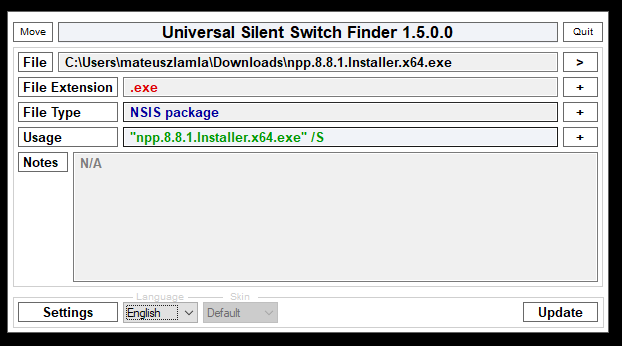
\includegraphics[width=0.8\linewidth]{media/USSF/1.PNG}
        \caption[]{Ekran główny programu (po wyborze ścieżki do instalatora możemy w polu Usage skopiować polecenie do wklejenia w cmd)}
        \label{fig:ussf_ekran_glowny}
    \end{figure}

    \begin{figure}[H]
        \centering
        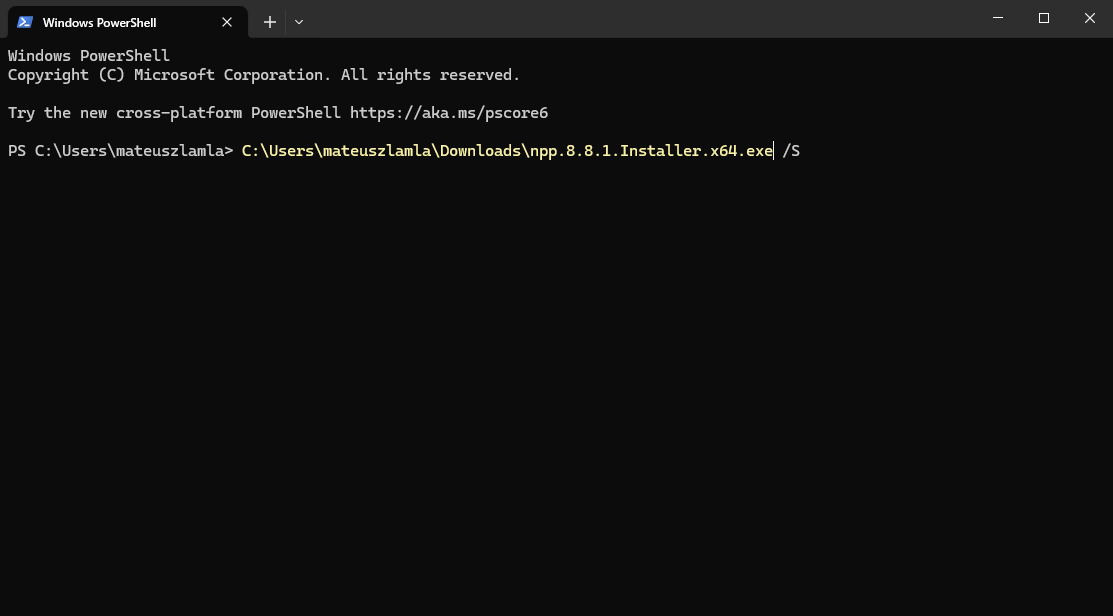
\includegraphics[width=0.8\linewidth]{media/USSF/2.PNG}
        \caption[]{Wykonanie skopiowanego wcześniej polecenia cichej instalacji}
        \label{fig:uusf_cicha_instalacja}
    \end{figure}

    \begin{figure}[H]
        \centering
        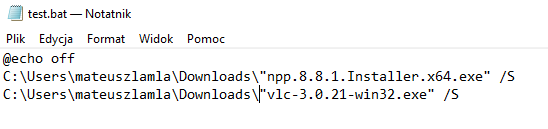
\includegraphics[width=0.8\linewidth]{media/USSF/3.PNG}
        \caption[]{Możemy również utworzyć skrypt wykonujący wiele poleceń cichej instalacji na raz aby usprawnić pracę}
        \label{fig:ussf_wiele_instalacji}
    \end{figure}
    
    \begin{figure}[H]
        \centering
        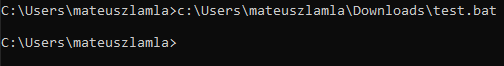
\includegraphics[width=0.8\linewidth]{media/USSF/4.PNG}
        \caption[]{Wykonanie pliku .bat z instalacjami}
        \label{fig:ussf_wykonanie_bat}
    \end{figure}

    \begin{figure}[H]
        \centering
        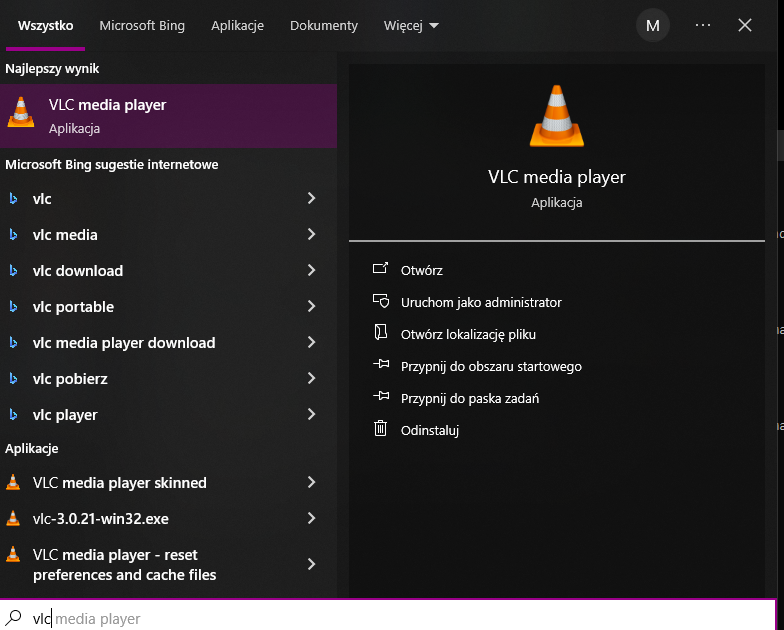
\includegraphics[width=0.8\linewidth]{media/USSF/5.PNG}
        \caption[]{Program zainstalowany}
        \label{fig:ussf_vlc_zainstalowane}
    \end{figure}

    \begin{figure}[H]
        \centering
        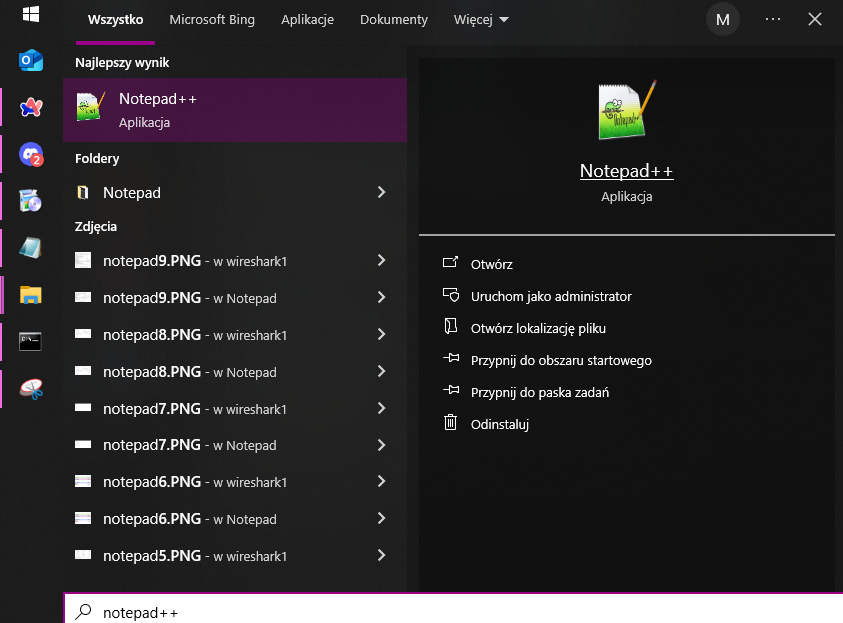
\includegraphics[width=0.8\linewidth]{media/USSF/6.PNG}
        \caption[]{Program zainstalowany}
        \label{fig:ussf_notepad++_zainstalowany}
    \end{figure}
\newpage    
    Innym programem pozwalającym na cichą instalację jest \textbf{Silent Install Helper}, który pozwala na tworzenie własnych cichych instalatorów.

\subsubsection{7-Zip}
    Lekkie i szybkie narzędzie do archiwizacji, wspierające wiele formatów.
    \begin{figure}[H]
        \centering
        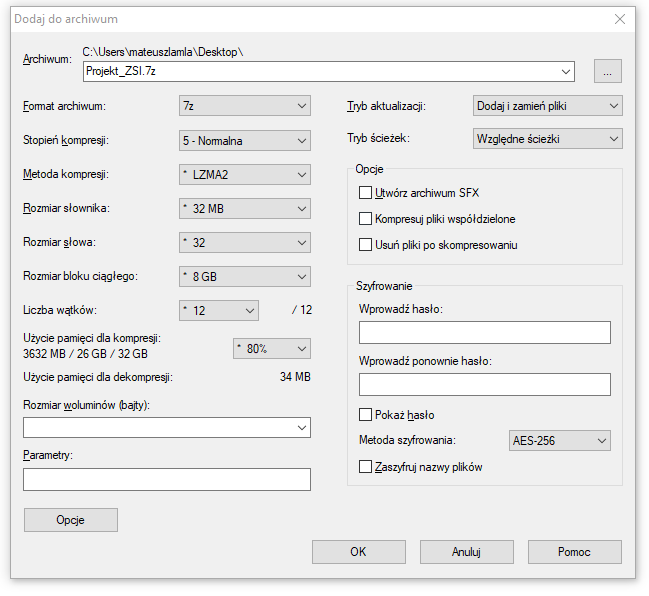
\includegraphics[width=0.8\linewidth]{media/7zip/1_kompresja_7z.PNG}
        \caption[]{Kompresja w formacie .7z}
        \label{fig:7z_kompresja_7z}
    \end{figure}

    \begin{figure}[H]
        \centering
        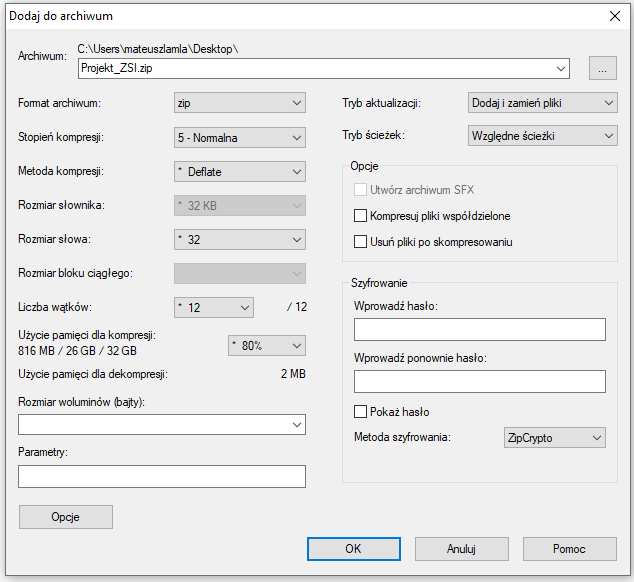
\includegraphics[width=0.8\linewidth]{media/7zip/2_kompresja_zip.PNG}
        \caption[]{Kompresja w formacie .zip}
        \label{fig:7z_kompresja_zip}
    \end{figure}

    \begin{figure}[H]
        \centering
        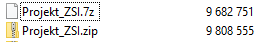
\includegraphics[width=0.8\linewidth]{media/7zip/3_porownanie_rozmiarow.PNG}
        \caption[]{Porównanie rozmiarów obu skompresowanych folderów. Kompresja .7z jest lepsza niż .zip}
        \label{fig:7z_porownanie_rozmiarow}
    \end{figure}

    \begin{figure}[H]
        \centering
        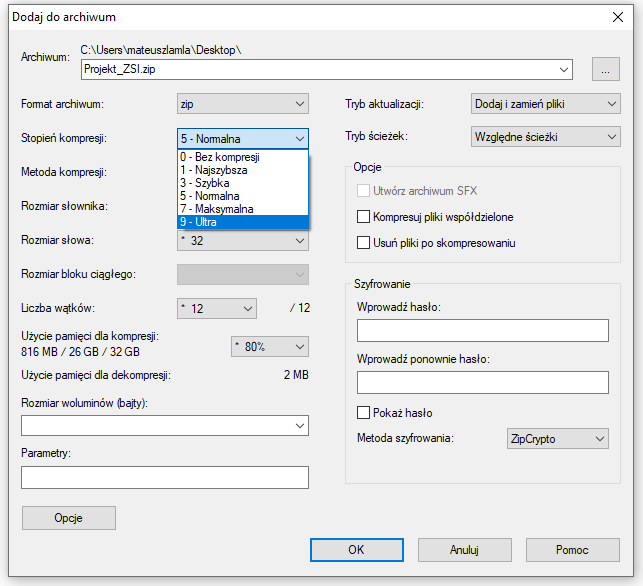
\includegraphics[width=0.8\linewidth]{media/7zip/4_poziom_kompresji.PNG}
        \caption[]{Możliwość wyboru poziomu kompresji}
        \label{fig:7z_poziom_kompresji}
    \end{figure}

    \begin{figure}[H]
        \centering
        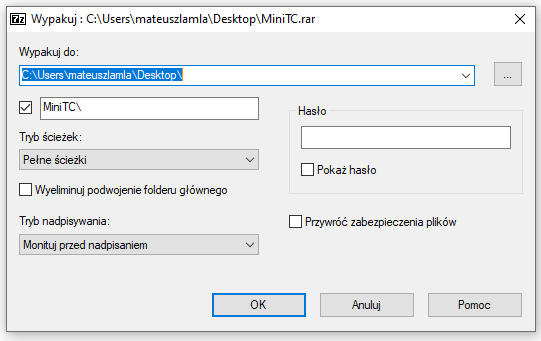
\includegraphics[width=0.8\linewidth]{media/7zip/5_wypakowywanie_innych_formatow_np_rar.PNG}
        \caption[]{Program 7zip umożliwia wypakowywanie folderów skompresowanych w innych formatach niż .7z np. .rar}
        \label{fig:7z_wypakowanie_rar}
    \end{figure}

    \begin{figure}[H]
        \centering
        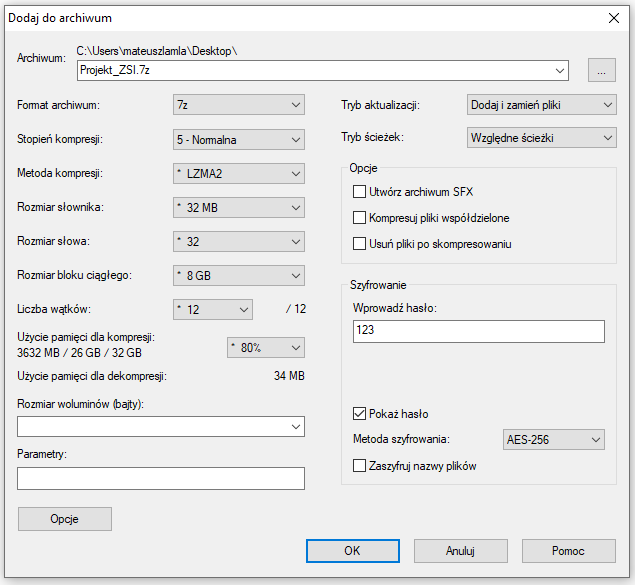
\includegraphics[width=0.8\linewidth]{media/7zip/6_mozliwosc_dodawania_hasla_do_archiwum.PNG}
        \caption[]{Istnieje również opcja zabezpieczenia folderu hasłem co jest bardzo przydatną funkcjonalnością szczególnie dla plików wrażliwych}
        \label{fig:7z_zabezpieczenie_haslem}
    \end{figure}

    \begin{figure}[H]
        \centering
        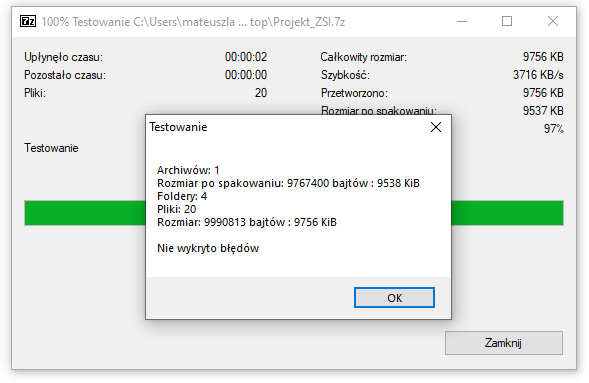
\includegraphics[width=0.8\linewidth]{media/7zip/7_testowanie_archiwow.PNG}
        \caption[]{Testowanie archiwów - sprawdzanie błedów}
        \label{fig:7z_testowanie_archiwow}
    \end{figure}

    \begin{figure}[H]
        \centering
        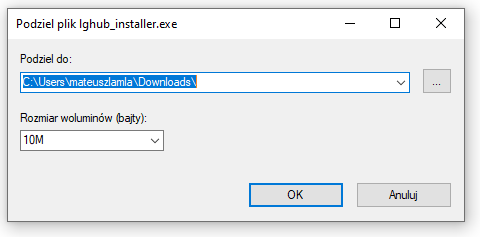
\includegraphics[width=0.8\linewidth]{media/7zip/8_dzielenie_plikow_na_mniejsze.PNG}
        \caption[]{Podział pliku na mniejsze. Przydatne przy plikach o dużych rozmiarach}
        \label{fig:7z_podzial_plik}
    \end{figure}

    \begin{figure}[H]
        \centering
        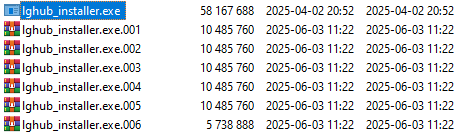
\includegraphics[width=0.8\linewidth]{media/7zip/9_podzielone_pliki.PNG}
        \caption[]{Podzielone pliki}
        \label{fig:7z_podzielone_pliki}
    \end{figure}

    \begin{figure}[H]
        \centering
        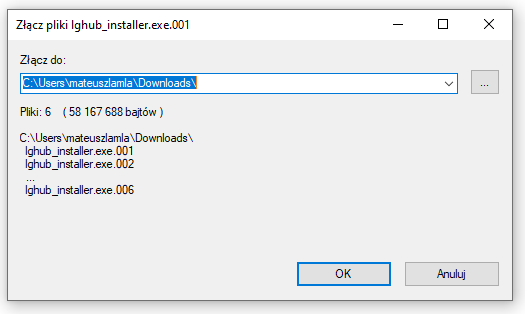
\includegraphics[width=0.8\linewidth]{media/7zip/10_zlaczanie_podzielonych_plikow.PNG}
        \caption[]{Łączenie podzielonych plików. Wcześniej podzielone pliki możemy teraz złączyć z powrotem w jeden}
        \label{fig:7z_laczenie_podzielonych_plikow}
    \end{figure}
    
    Innym programem może być \textbf{WinRAR}, który jest nieco bardziej przyjazny dla zwykłego użytkownika, jednak jest on płatny.
\newpage
\subsubsection{Wireshark}
    Analizator pakietów sieciowych. Kluczowe narzędzie do diagnozowania problemów z siecią lub analizowania ruchu sieciowego na naszych interfejsach.

    \begin{figure}[H]
        \centering
        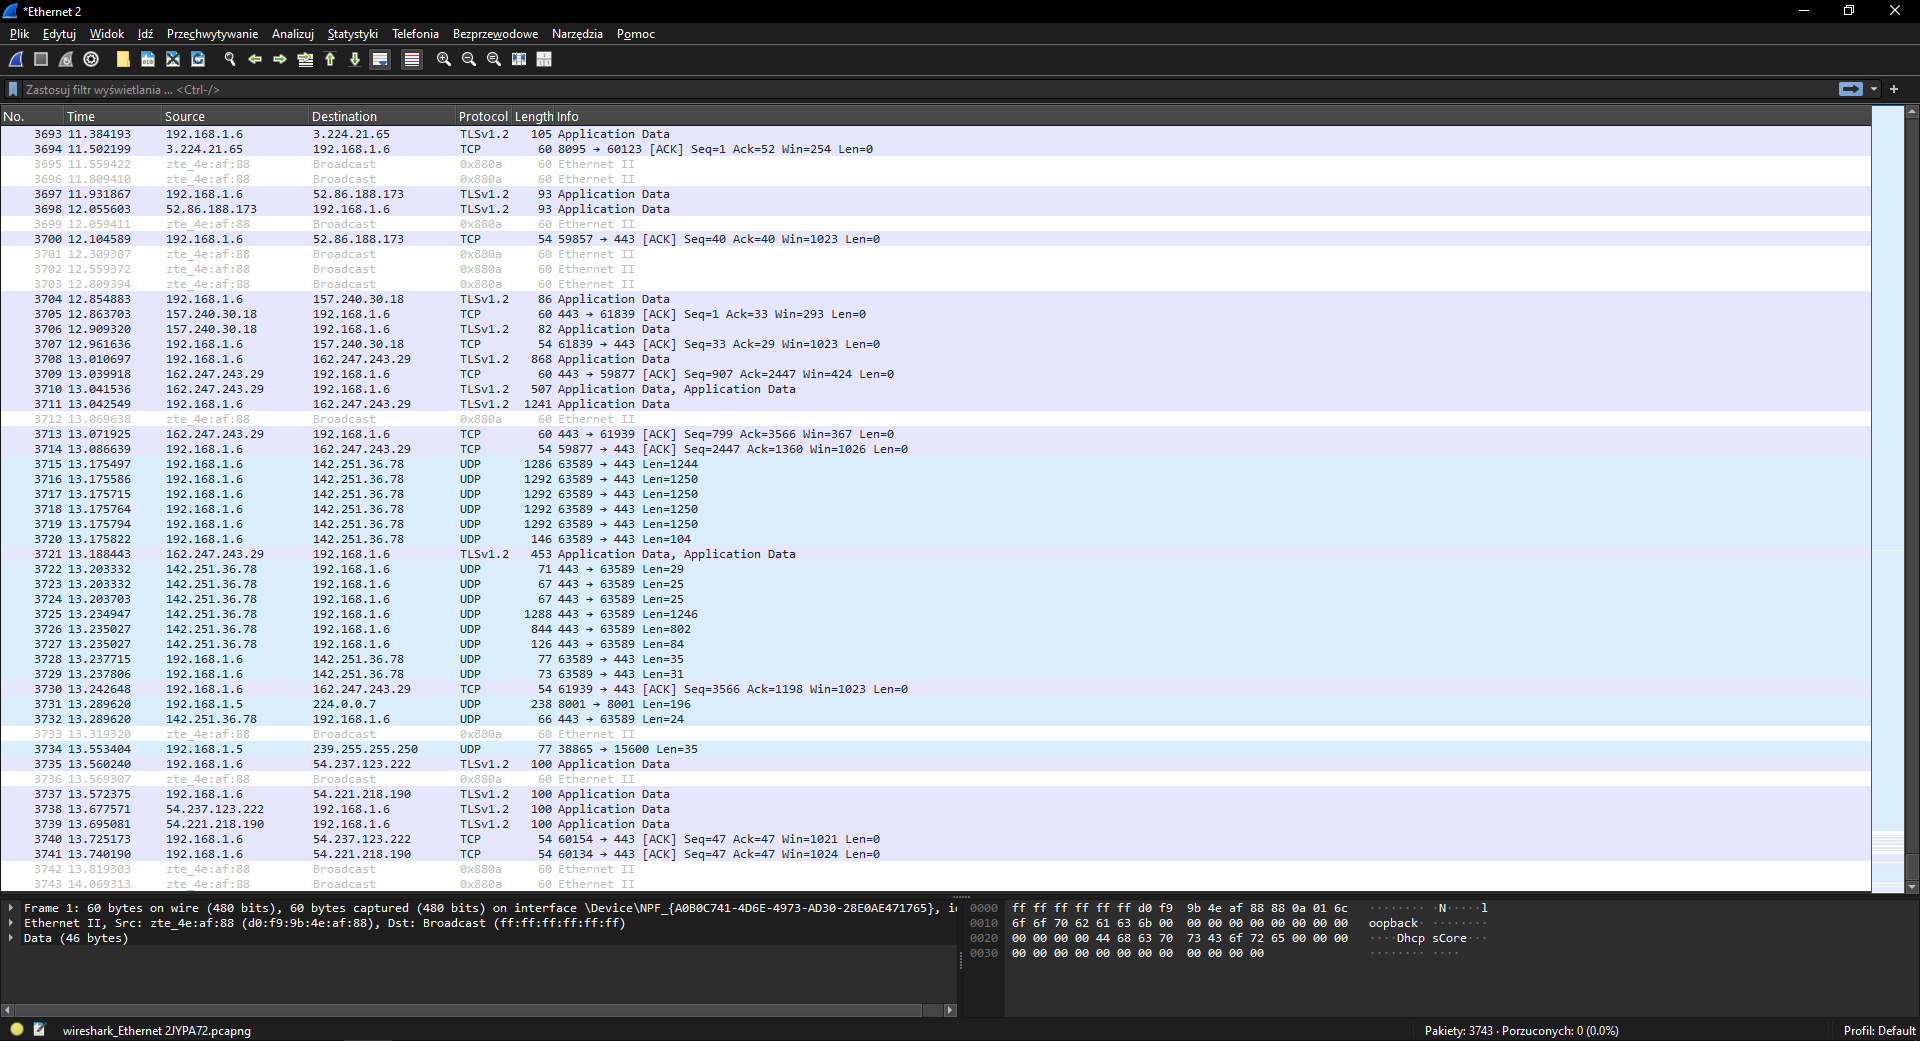
\includegraphics[width=0.8\linewidth]{media/Wireshark/wireshark1.PNG}
        \caption[wireshark glowne]{Połączenie z interfejsem sieciowym.}
        \label{fig:wire_polaczenie}
    \end{figure}

    \begin{figure}[H]
        \centering
        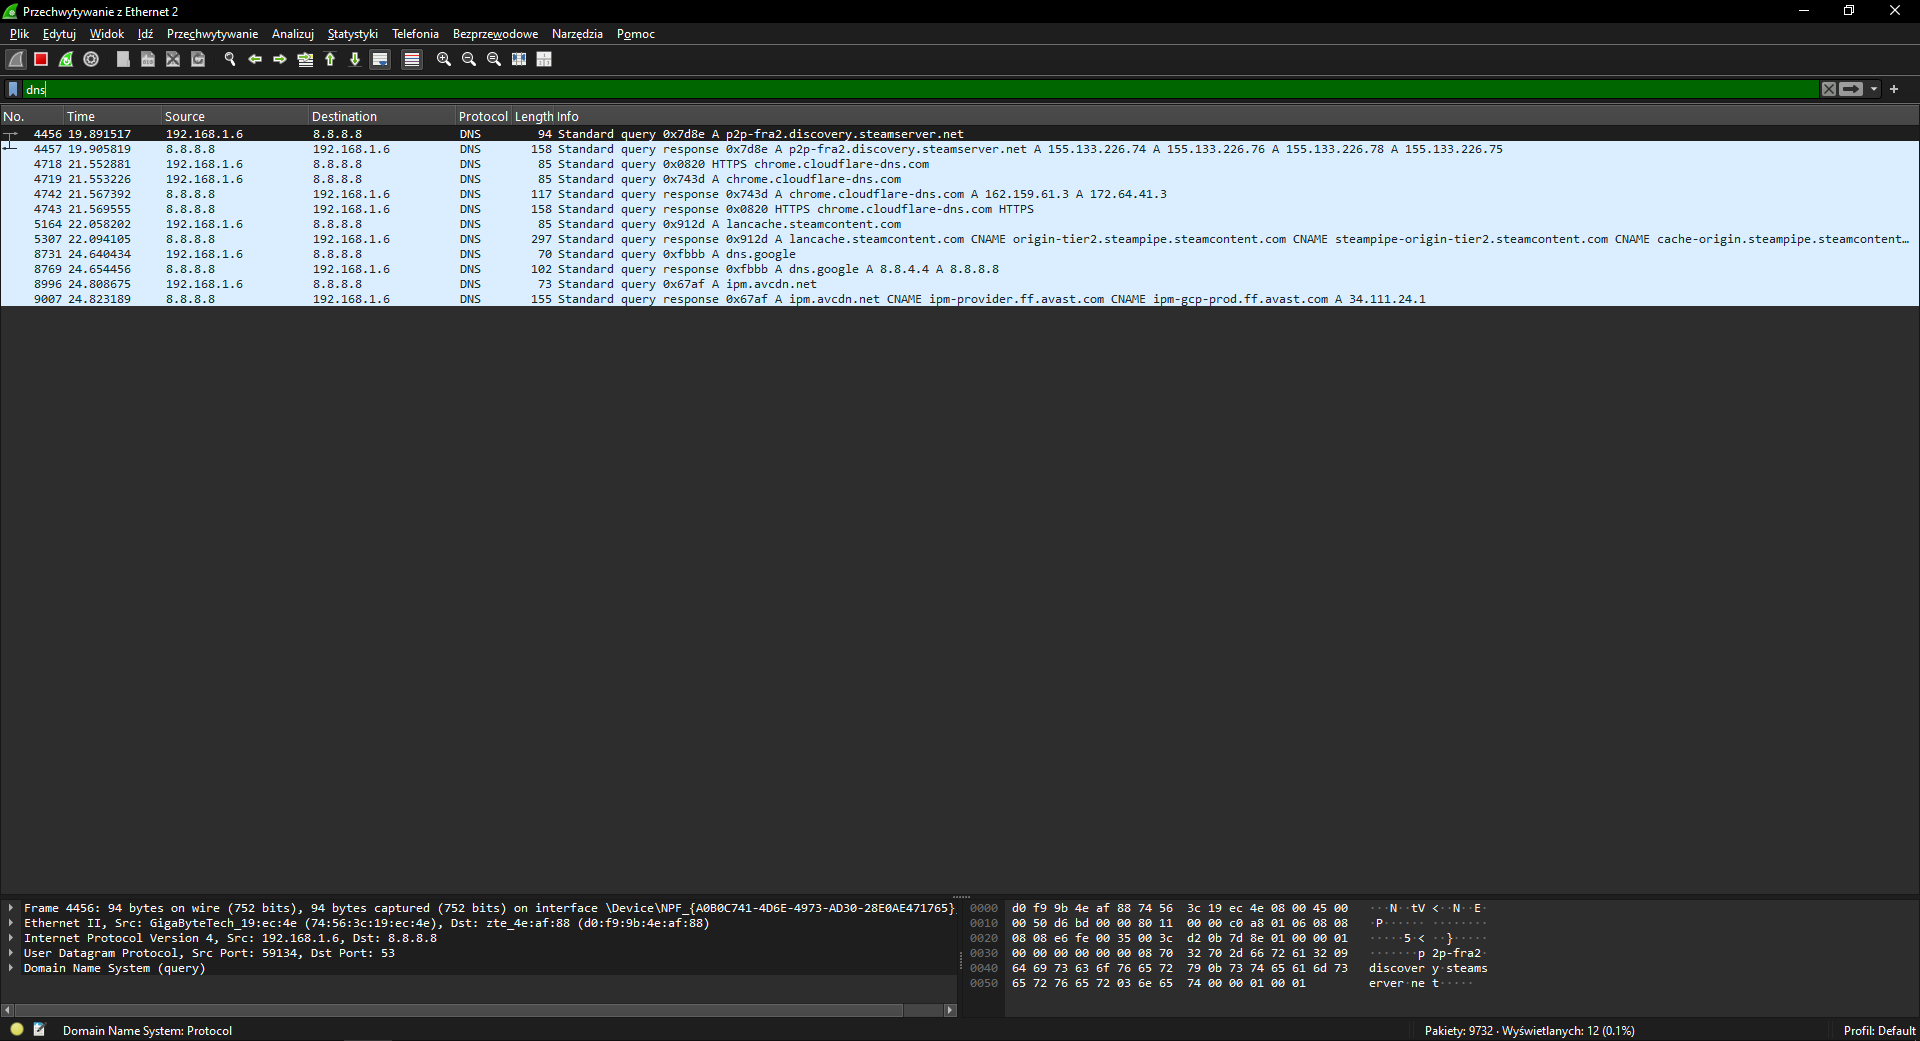
\includegraphics[width=0.8\linewidth]{media/Wireshark/wireshark2_dns.PNG}
        \caption[wireshark filtr]{Możliwość filtrowania pakietów po protokole sieciowym.}
        \label{fig:wireshark_dns}
    \end{figure}

    \begin{figure}[H]
        \centering
        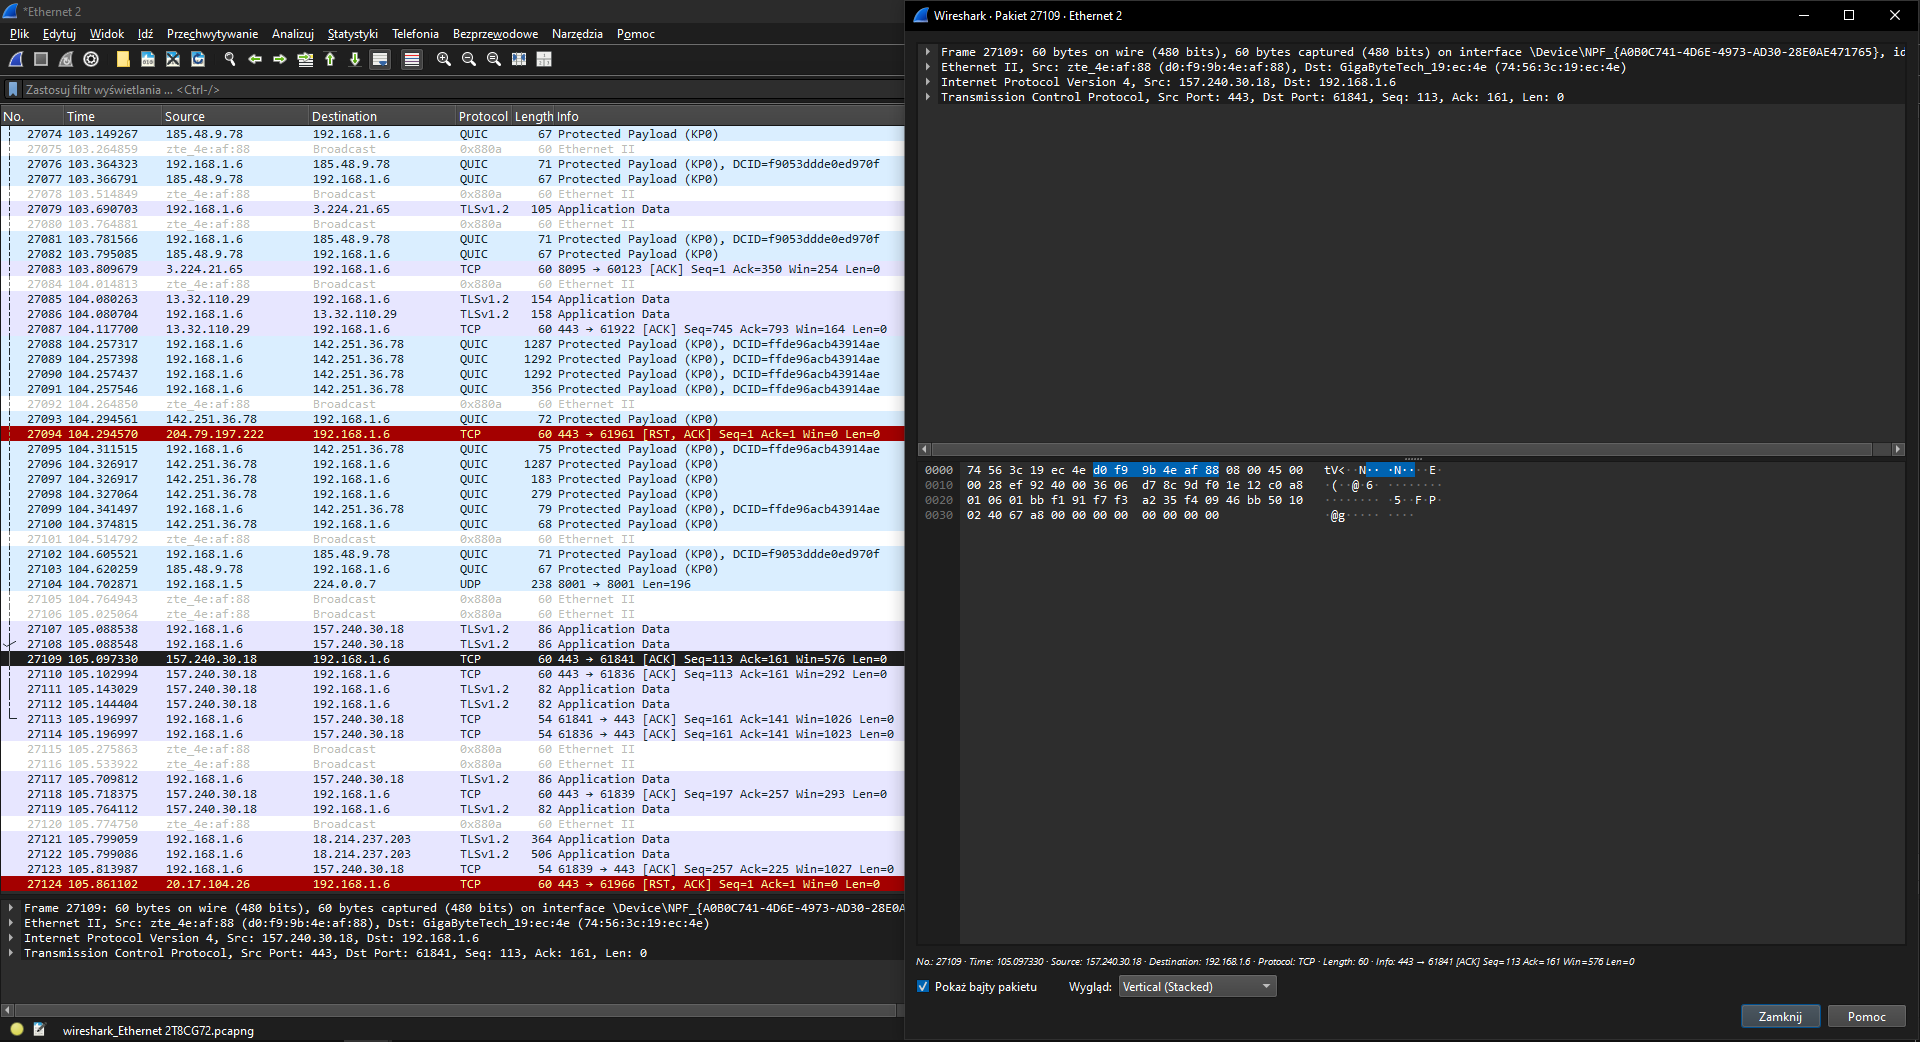
\includegraphics[width=0.8\linewidth]{media/Wireshark/wireshark3.PNG}
        \caption[wireshark szczegoly]{Możliwość wybrania pakietu do wyświetlenia jego szczegółów.}
        \label{fig:wireshark_klik}
    \end{figure}

    \begin{figure}[H]
        \centering
        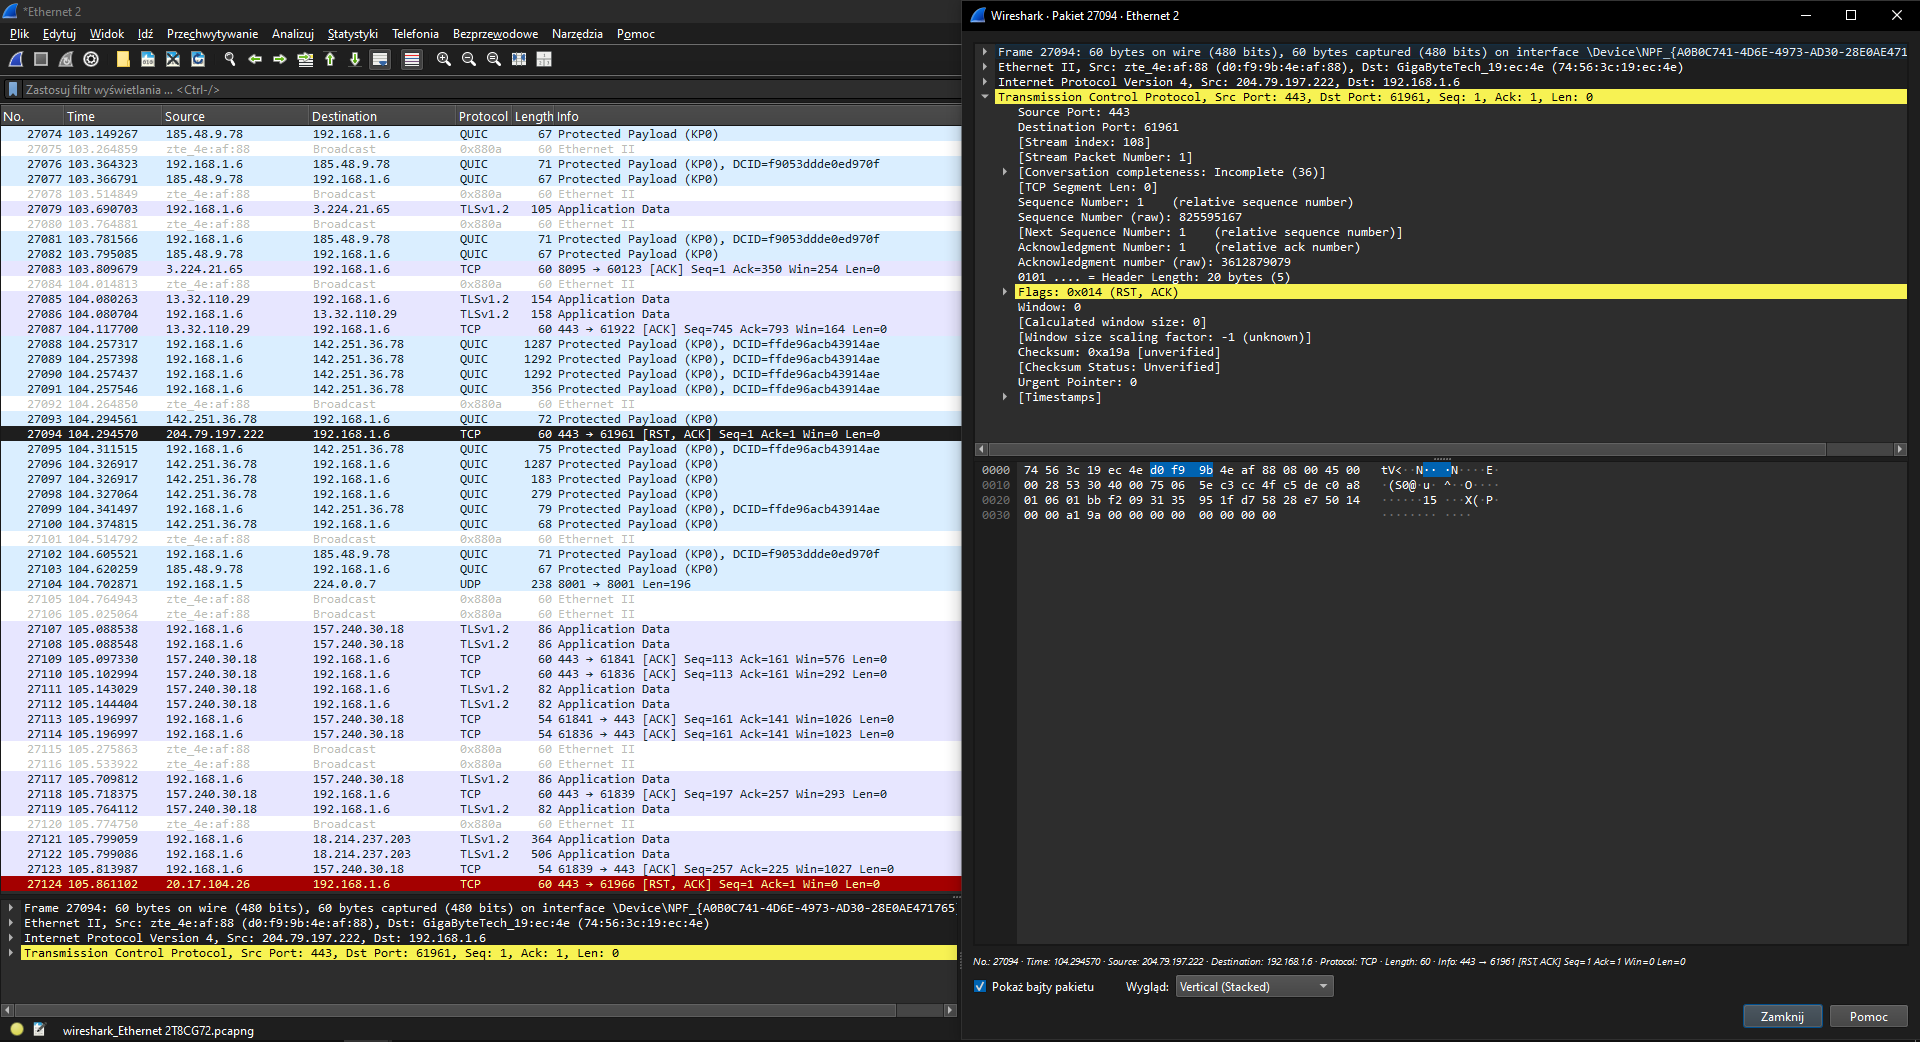
\includegraphics[width=0.8\linewidth]{media/Wireshark/wireshark4_odrzucone.PNG}
        \caption[wireshark odrzucone]{Po rozwinięciu wybranego pakietu i zakładki protokołu, mamy rozpisane szczegółowe informacje o pakiecie takie jak np. flagi. W przypadku powyższego zrzutu ekranu widać, że próba dostarczenia pakietu została przez jedną ze stron przerwana (RST).}
        \label{fig:wireshark_odrzucone}
    \end{figure}
    Wireshark jest naszym zdaniem najlepszym dostępnym narzędziem do analizy ruchu sieciowego, ale jako jego konkurenta można wspomnieć o \textbf{Capsa Network Analyzer}. Capsa kusi swoją łatwością obsługi oraz interfejsem, ale jest bardzo ograniczona w swojej darmowej wersji. Wireshark zapewnia pełen dostęp do szczegółów ruchu w sieci oraz jest całkowicie darmowy.
\newpage
\subsubsection{Notepad++}
    Rozbudowany edytor tekstu, przydatny do edycji plików konfiguracyjnych, skryptów i logów. Obsługuje wiele rozszerzeń plików, dzięki czemu bez problemu możemy używać go do zróżnicowanych projektów bez obaw, że nie będzie on wspierał używanego przez nas języka lub typu pliku.

    \begin{figure}[H]
        \centering
        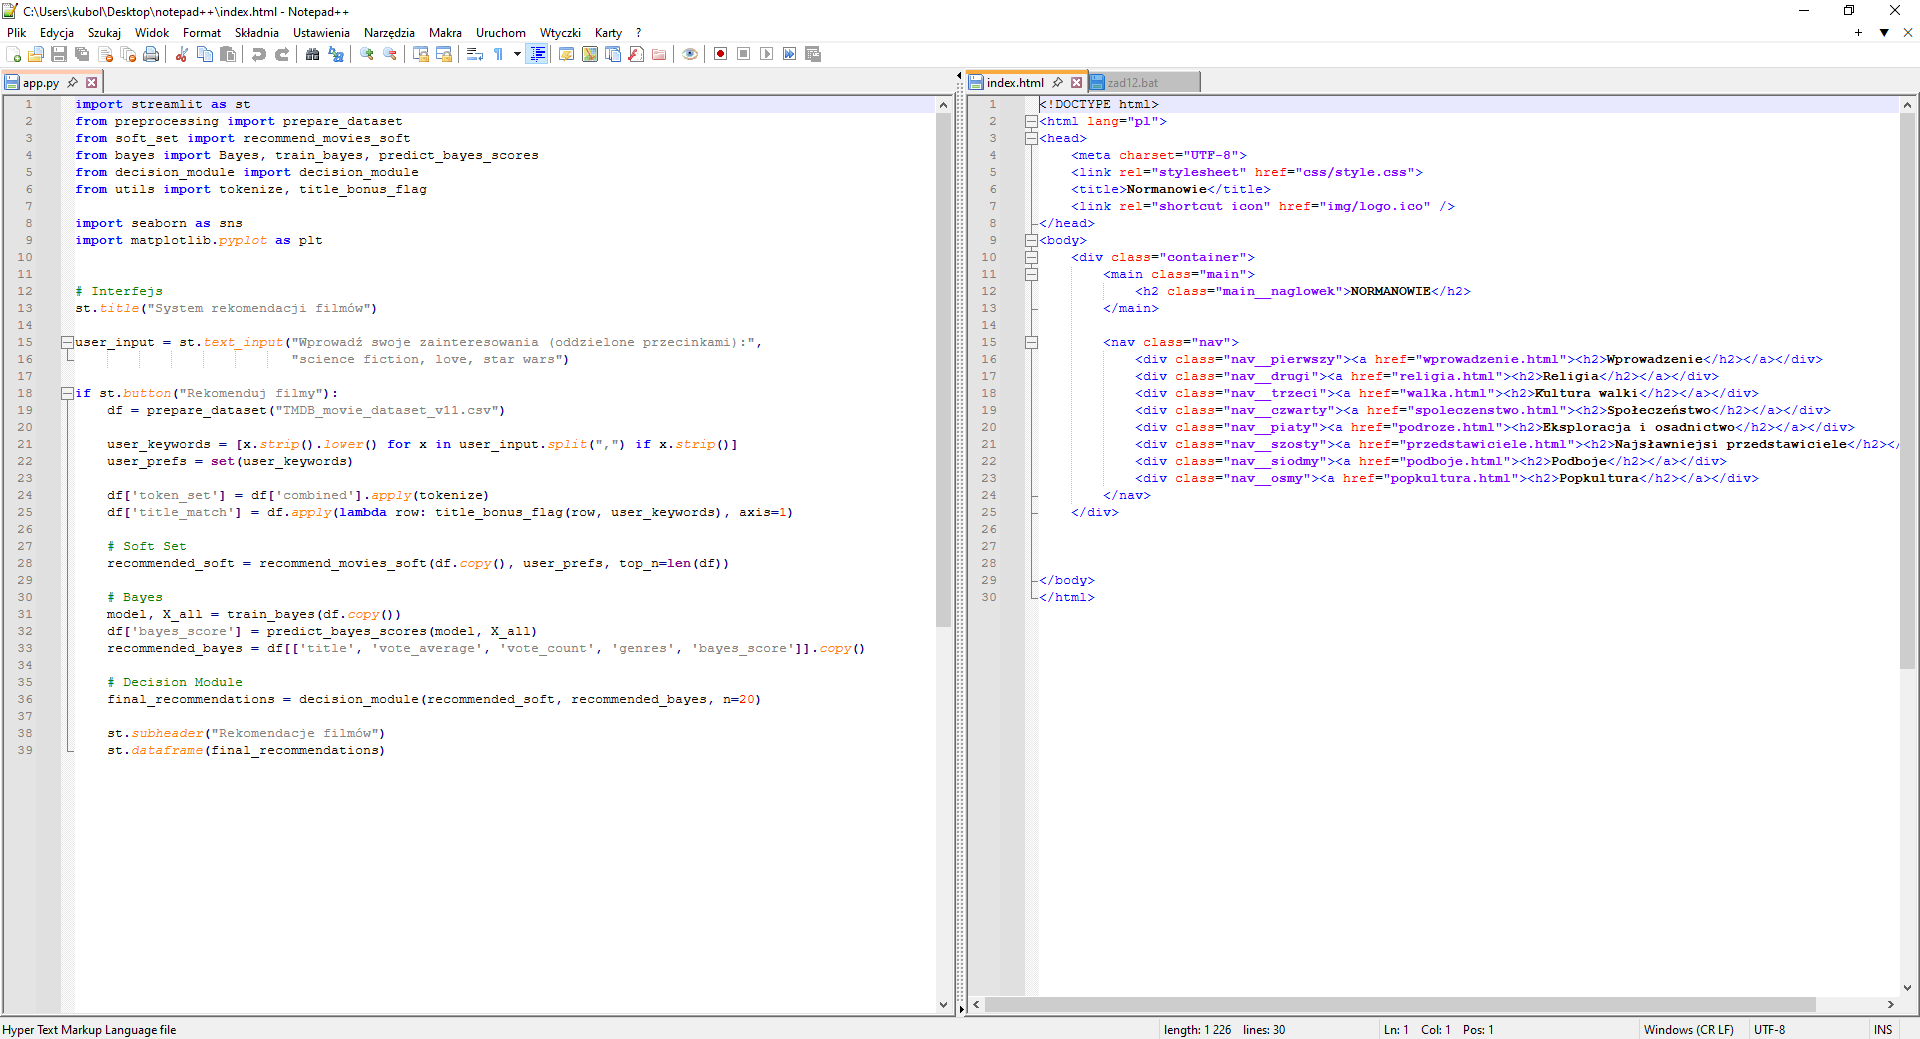
\includegraphics[width=0.8\linewidth]{media/Notepad/notepad1.PNG}
        \caption[notepad glowne]{Wyświetlenie dwóch plików z całkowicie różnymi rozszerzeniami. Jak widać, w obu plikach mamy podświetlanie składni, co ułatwia modyfikacje plików.}
        \label{fig:notepad_glowne}
    \end{figure}

    \begin{figure}[H]
        \centering
        \includegraphics[width=0.8\linewidth]{media/Notepad/notepad2.png}
        \caption[notepad zapis]{Przy okazji zapisu pliku utworzonego w programie mamy rozbudowaną listę rozszerzeń, w jakich możemy taki plik zapisać. Program obsługuje dziesiątki możliwych typów plików.}
        \label{fig:}
    \end{figure}

    \begin{figure}[H]
        \centering
        \includegraphics[width=0.8\linewidth]{media/Notepad/notepad3.png}
        \caption[notepad podpowiedzi]{Program oferuje również autouzupełnianie, co przyspiesza pracę użytkownikowi i wspomaga w przypadku zapomnienia słów kluczowych używanych w danym języku.}
        \label{fig:notepad_podpowiedzi}
    \end{figure}

    \begin{figure}[H]
        \centering
        \includegraphics[width=0.8\linewidth]{media/Notepad/notepad4.png}
        \caption[notepad wyszukiwanie]{Notepad++ umożliwia wyszukiwanie słów w plikach znajdujących się w wybranym folderze. Dodatkowo daje opcję zamieniania wyrażeń w plikach na inne w tym samym okienku (zakładka obok).}
        \label{fig:notepad_wyszukiwanie}
    \end{figure}

    \begin{figure}[H]
        \centering
        \includegraphics[width=0.8\linewidth]{media/Notepad/notepad5.PNG}
        \caption[notepad info]{Program zapewnia łatwy dostęp do szczegółowych informacjach o pliku, takich jak ilość słów lub co zostało zaznaczone przez użytkownika.}
        \label{fig:notepad_info}
    \end{figure}

    \begin{figure}[H]
        \centering
        \includegraphics[width=0.8\linewidth]{media/Notepad/notepad6.PNG}
        \caption[notepad kolory]{W celu zwiększenia przejrzystości plików oraz ich organizacji, program zapewnia opcję wyróżniania plików na wybrane kolory w swoim bocznym panelu odpowiadającemu za eksplorator plików.}
        \label{fig:notepad_kolory}
    \end{figure}

    \begin{figure}[H]
        \centering
        \includegraphics[width=0.8\linewidth]{media/Notepad/notepad7.PNG}
        \caption[notepad html]{Każdy z plików można za pomocą jednego przycisku przekonwertować na stronę html wraz z podświetleniem składni zgodnym z oryginalnym rozszerzeniem pliku.}
        \label{fig:notepad_html}
    \end{figure}

    \begin{figure}[H]
        \centering
        \includegraphics[width=0.8\linewidth]{media/Notepad/notepad8.PNG}
        \caption[notepad podswietlenie kolory]{Podświetlenie składni możemy modyfikować zależnie od naszych upodobań za pomocą wbudowanego konfiguratora stylów.}
        \label{fig:notepad_kolory_skladnia}
    \end{figure}

    \begin{figure}[H]
        \centering
        \includegraphics[width=0.8\linewidth]{media/Notepad/notepad9.PNG}
        \caption[notepad skroty]{Program zapewnia też modyfikacje skrótów klawiszowych, aby usprawnić płynność prac nad projektami użytkownika za pomocą dostosowania się do jego przyzwyczajeń klawiszowych.}
        \label{fig:notepad_skroty}
    \end{figure}

    Największym konkurentem dla Notepad++ jest \textbf{VS Code}. Wybrany przez nas program góruje nad swoją alternatywą przede wszystkim swoją szybkością i lekkością. Nadaje się idealnie do szybkiej i wygodnej edycji plików bez uruchamiania całego IDE. Pomimo, że nie jest on tak rozbudowany jak VS Code, uznaliśmy go za dużo lepszą opcję dla administratora.
\newpage
\subsubsection{Windows Terminal}
    Nowoczesna konsola obsługująca PowerShell, CMD i WSL. Pozwala zintegrować wiele powłok w jednym środowisku.

    \begin{figure}[H]
        \centering
        \includegraphics[width=0.8\linewidth]{media/Windows Terminal/1_wiele_kart.PNG}
        \caption[]{Możliwość dzielenia ekranu}
        \label{fig:terminal_dzielenie_ekranu}
    \end{figure}

    \begin{figure}[H]
        \centering
        \includegraphics[width=0.8\linewidth]{media/Windows Terminal/2_mozliwosc_personalizacji_wygladu.PNG}
        \caption[]{Program oferuje wiele opcji personalizacji wyglądu}
        \label{fig:terminal_presonalizacja}
    \end{figure}
    
    \begin{figure}[H]
        \centering
        \includegraphics[width=0.8\linewidth]{media/Windows Terminal/3_mozliwosc_korzystania_z_dwoch_systemow.PNG}
        \caption[]{Istnieje możliwość korzysta z kilku systemów operacyjnych równolegle}
        \label{fig:terminal_dwa_systemy}
    \end{figure}

    \begin{figure}[H]
        \centering
        \includegraphics[width=0.8\linewidth]{media/Windows Terminal/3_1_dostep do danych na jednym systemie z drugiego.PNG}
        \caption[]{Jest również opcja aby dostać się do danych z jednego systemu na drugim}
        \label{fig:terminal_dostep_miedzy_systemami}
    \end{figure}

    \begin{figure}[H]
        \centering
        \includegraphics[width=0.8\linewidth]{media/Windows Terminal/4_command_palette.PNG}
        \caption[]{Paleta komend}
        \label{fig:terminal_paleta_komend}
    \end{figure}

    \begin{figure}[H]
        \centering
        \includegraphics[width=0.8\linewidth]{media/Windows Terminal/5_wyszukiwarka.PNG}
        \caption[]{Możemy wyszukać słowa kluczowe}
        \label{fig:terminal_wyszukiwarka}
    \end{figure}

    \begin{figure}[H]
        \centering
        \includegraphics[width=0.8\linewidth]{media/Windows Terminal/6_klikalne_linki.PNG}
        \caption[]{Dużym ułatwieniem są klikalne linki których nie trzeba kopiować, a wystarczy kliknąć i przeniesie nas do odpowiedniej lokalizacji}
        \label{fig:terminal_klikalne_lnki}
    \end{figure}

    \begin{figure}[H]
        \centering
        \includegraphics[width=0.8\linewidth]{media/Windows Terminal/7_utworzenie_nowego_profilu_w_settings.png}
        \caption[]{Możemy również utworzyć nowy profil}
        \label{fig:terminal_nowy_profil}
    \end{figure}

    \begin{figure}[H]
        \centering
        \includegraphics[width=0.8\linewidth]{media/Windows Terminal/7_1nowy_profil_utworzony.PNG}
        \caption[]{Nowy profil w liście}
        \label{fig:terminal_nowy_profil}
    \end{figure}

    \begin{figure}[H]
        \centering
        \includegraphics[width=0.8\linewidth]{media/Windows Terminal/7_2_dzialajacy profil.PNG}
        \caption[]{Wejście do nowego profilu}
        \label{fig:terminal_nowy_profil_wejscie}
    \end{figure}
    
    Alternatywnym wyborem może być \textbf{ConEmu} posiadający dużą ilość możliwości konfiguracyjnych jednak mniej przyjazny interfejs od Windows Terminal.

\newpage
\subsubsection{OpenVPN}
    Narzędzie do konfiguracji bezpiecznych połączeń VPN. Umożliwia zdalny dostęp do zasobów firmowych.
    
    \begin{figure}[H]
        \centering
        \includegraphics[width=0.8\linewidth]{media/OpenVPN/0_logowanie.PNG}
        \caption[]{Strona logowania}
        \label{fig:vpn_strona_logowania}
    \end{figure}

    \begin{figure}[H]
        \centering
        \includegraphics[width=0.8\linewidth]{media/OpenVPN/1_IP_przed_VPN.PNG}
        \caption[]{Adres IP przed połączeniem VPN}
        \label{fig:vpn_ip_przed_vpn}
    \end{figure}
 
    \begin{figure}[H]
        \centering
        \includegraphics[width=0.8\linewidth]{media/OpenVPN/2_polaczenie_z_serwerem.PNG}
        \caption[]{Połączenie z serwerem VPN}
        \label{fig:vpn_polaczenie_z_serwerem}
    \end{figure}
        
    \begin{figure}[H]
        \centering
        \includegraphics[width=0.8\linewidth]{media/OpenVPN/3_zmiana_adresu_IP.PNG}
        \caption[]{Adres IP po połączeniu z VPN}
        \label{fig:vpn_ip_po_vpn}
    \end{figure}
        
    \begin{figure}[H]
        \centering
        \includegraphics[width=0.8\linewidth]{media/OpenVPN/4_logi.PNG}
        \caption[]{Możliwość sprawdzenia logów}
        \label{fig:vpn_logi}
    \end{figure}
    
    Alternatywą może być \textbf{WireGuard}, który skupia się na szybkości i bezpieczeństwie, jednak jest mniej rozbudowany.
\newpage   
\subsubsection{Clonezilla}
    Narzędzie do tworzenia i przywracania obrazów dysków. Wsparcie przy migracjach systemów i backupach. W celu przedstawienia działania programu zrobiliśmy kopię partycji i przywróciliśmy ją do innej partycji.

    \begin{figure}[H]
        \centering
        \includegraphics[width=0.8\linewidth]{media/Clonezilla/clone1.PNG}
        \caption[clone 1]{Przygotowanie partycji do procesu klonowania i przywracania. W tym przypadku partycja (D:) wraz z jej zawartością będzie klonowana i przywracana do partycji (E:).}
        \label{fig:clone1}
    \end{figure}
    
    \begin{figure}[H]
        \centering
        \includegraphics[width=0.8\linewidth]{media/Clonezilla/clone2.PNG}
        \caption[clone glowne]{Ekran bootowania programu po restarcie maszyny i zamontowaniu obrazu Clonezilli.}
        \label{fig:clone2}
    \end{figure}
    
    \begin{figure}[H]
        \centering
        \includegraphics[width=0.8\linewidth]{media/Clonezilla/clone3.PNG}
        \caption[clone start]{Program po załadowaniu daje nam możliwość uruchomienia Clonezillę lub przejście do wiersza poleceń.}
        \label{fig:clone3}
    \end{figure}
    
    \begin{figure}[H]
        \centering
        \includegraphics[width=0.8\linewidth]{media/Clonezilla/clone4.PNG}
        \caption[clone wybor opcji]{Program daje nam do wyboru różne opcje klonowania jak np. urządzenie do obrazu czy urządzenie do urządzenia bezpośrednio. Nas interesuje opcja z obrazami na potrzeby prezentacji działania programu.}
        \label{fig:clone4}
    \end{figure}
    
    \begin{figure}[H]
        \centering
        \includegraphics[width=0.8\linewidth]{media/Clonezilla/clone5.PNG}
        \caption[clone dyskpart]{Clonezilla umożliwia nam zarówno klonowanie całości dysku lub jedynie jego częsci w postaci partycji.}
        \label{fig:clone5}
    \end{figure}
    
    \begin{figure}[H]
        \centering
        \includegraphics[width=0.8\linewidth]{media/Clonezilla/clone6.PNG}
        \caption[clone lista]{Każda z partycji jest dokładnie opisana przy wyborze do utworzenia klona. Widzimy rozmiar, numer, system plików oraz etykiety.}
        \label{fig:clone6}
    \end{figure}
    
    \begin{figure}[H]
        \centering
        \includegraphics[width=0.8\linewidth]{media/Clonezilla/clone7.PNG}
        \caption[clone gdzie]{Po wyborze partycji do sklonowania znika nam ona z możliwych miejsc docelowych klonowania.}
        \label{fig:clone7}
    \end{figure}
    
    \begin{figure}[H]
        \centering
        \includegraphics[width=0.8\linewidth]{media/Clonezilla/clone8.PNG}
        \caption[clone naprawa]{Program daje możliwość sprawdzenia jeszcze przed procesem klonowania systemy plików obu partycji, aby zapobiec niechcianym błędom.}
        \label{fig:clone8}
    \end{figure}
    
    \begin{figure}[H]
        \centering
        \includegraphics[width=0.8\linewidth]{media/Clonezilla/clone9.PNG}
        \caption[clone wylaczenie]{Klasycznie dla programów tego typu daje nam on możliwość zrestartowania maszyny po całym procesie, aby wszystko mogło się na nowo załadować i działać od razu bez problemów.}
        \label{fig:clone9}
    \end{figure}
    
    \begin{figure}[H]
        \centering
        \includegraphics[width=0.8\linewidth]{media/Clonezilla/clone10.PNG}
        \caption[clone zapytania]{Po wybraniu wszystkich opcji program wielokrotnie pyta nas, czy na pewno chcemy wykonać klona na daną partycję. Jest to spowodowane nadpisywaniem danych na wybranej partycji.}
        \label{fig:clone10}
    \end{figure}
    
    \begin{figure}[H]
        \centering
        \includegraphics[width=0.8\linewidth]{media/Clonezilla/clone11.PNG}
        \caption[clone koniec]{Po zaakceptowaniu procesu klonowania program przechodzi do działania. Ze względu na to, że zawartość partycji była skromna, to program uporał się z tym w zaledwie pare sekund.}
        \label{fig:clone11}
    \end{figure}
    
    \begin{figure}[H]
        \centering
        \includegraphics[width=0.8\linewidth]{media/Clonezilla/clone12.PNG}
        \caption[clone restart]{Po udanym wykonaniu klona, możemy wybrać co chcemy zrobić dalej. Najwygodniej jest zrestartować maszynę i wrócić do naszego systemu operacyjnego.}
        \label{fig:clone12}
    \end{figure}
    
    \begin{figure}[H]
        \centering
        \includegraphics[width=0.8\linewidth]{media/Clonezilla/clone13.PNG}
        \caption[clone rezultat]{Jak widać, sklonowana została etykieta partycji oraz zawartość, nie zmieniając przy tym jednak ogólnego rozmiaru partycji.}
        \label{fig:clone13}
    \end{figure}
    
    \begin{figure}[H]
        \centering
        \includegraphics[width=0.8\linewidth]{media/Clonezilla/clone14.PNG}
        \caption[clone prezentacja]{W formie prezentacji rezultatu klonowania widać, że pliki pojawiły się na partycji pierwotnie przeznaczonej do przywrócenia klona.}
        \label{fig:clone14}
    \end{figure}
    Najczęściej polecaną alternatywą dla Clonezilli jest \textbf{Macrium Reflect}. Pomimo posiadania graficznego interfejsu i działania z poziomu systemu Windows, nie jest on tak jak Clonezilla programem otwartoźródłowym. Macrium oferuje okrojoną wersję Trial oraz pełną płatną wersję. Clonezilla dodatkowo oferuje obsługę innych systemów niż Windows oraz większą gamę systemów plików. Dodatkowo wybrany przez nas program jest znacznie lżejszy, z powodu interfejsu tekstowego, jednocześnie posiadając więcej opcji.

\newpage
\section{Klasyfikacja programów}
    Po przenalizowaniu funkcjonalności każdego z zaproponowanych programów, sklasyfikowaliśmy ich użyteczność w postaci rankingu 1-10:
    \begin{enumerate}
        \item \textbf{OpenSSH} -- Program niezbędny do zdalengo zarządzania systemami, co jest kluczowe w pracy administratora.
        \item \textbf{Wireshark} -- Niezastąpiony w analize ruchu sieciowego.
        \item \textbf{Everything (Voidtools)} -- Pozwala błyskawicznie wyszukać pożądany plik nawet w najbardziej zapełnionych dyskach.
        \item \textbf{7-Zip} -- Zapewnia obsługę prawie wszystkich formatów kompresji będąc przy tym skryptowalnym i szybkim.
        \item \textbf{Windows Terminal} -- wygodna konsola, która posiada wiele funkcjonalności ułatwiających pracę z wieloma systemami na raz.
        \item \textbf{Notepad++} -- Szybki i lekki edytor tekstu z wieloma opcjami personalizacji oraz obsługiwanymi rozszerzeniami plików.
        \item \textbf{Clonezilla} -- Najlepszy program do tworzenia backupów, masowego wdrażania systemów oraz ratowania niesprawnych systemów. Wymaga sporej wprawy od użytkownika.
        \item \textbf{WizTree} -- Bardzo szybkie narzędzie do dokładnego skanowania dysku. Nie jest on jednak przydatny w codziennej pracy, tylko w przypadku nagłej potrzeby.
        \item \textbf{OpenVPN} -- Świetny do tworzenia tuneli VPN. Program bardziej niszowy, niewykorzystywany przez wielu administratorów.
        \item \textbf{USSF} -- Program użyteczny w razie potrzeby instalacji wielu programów na wielu systemach, najrzadziej wykorzystywane w codziennej pracy administratora.
    \end{enumerate}
\section{Wnioski}
	\begin{itemize}
		\item \textit{Spostrzeżenia:} Każde z analizowanych narzędzi spełnia swoją funkcję, ich użyteczność w dużym stopniu zależy od środowiska pracy administratora. Jednak narzędzia takie jak Notepad++ czy OpenSSH stanowią fundament codziennej pracy.
		\item \textit{Osiągnięcia:} Udało się przetestować najpopularniejsze programy dla administratorów i porównać je w jednolity sposób.
		\item \textit{Potencjał rozwoju:} Możliwe jest rozszerzenie projektu o kolejne narzędzia, a także o ich ocenę pod kątem innych systemów.
	\end{itemize}

\newpage
\section{Bibliografia}
\begin{enumerate}
	\item \url{https://clonezilla.org/}
    \item \url{https://www.wireshark.org/}
    \item \url{https://www.voidtools.com/}
    \item \url{https://diskanalyzer.com/}
    \item \url{https://notepad-plus-plus.org/}
    \item \url{https://openvpn.net/}
    \item \url{https://www.7-zip.org/}
    \item \href{https://www.capstanservices.com/tools-blog/2018/4/4/the-ultimate-silent-switch-finder-ussf}{https://www.capstanservices.com}
    \item \url{https://apps.microsoft.com/detail/9n0dx20hk701?hl=pl-PL&gl=PL}
    \item \url{https://www.reddit.com/r/sysadmin/ }
    \item \url{https://attuneops.io/system-administrator-tools/#2025s_Updates_to_the_Tools}
\end{enumerate}

\end{document}